%%%%%%%%%%%%%%%%%%%%%%%%%%%%%%%%%%%%%%%%%%%%%%%%
\input{./format/preamble.ltx} 

%%%%%%%%%%%%%%%%%%%%%%%%%%%%%%%%%%%%%%%%%%%%%%%%
% as needed, comment the following lines by prefixing the percent sign (%) at the start of the line

\Drafttrue % comment to disable putting some guides in the draft form of the document

\PutLineNumberstrue % comment to disable line numbers and certain  preparation guides 

\Figurestrue % comment to disable the rendering figures

\GroupIDtrue % comment to disable group ID

\ResultDiscusstrue % comment to disable results and discussions

\Conctrue % comment to disable conclusions

%\Finishedtrue % comment to disable manuscript for final defense or binding/submission

%\ApprovalSheetSignedtrue % comment to disable inclusion of the signed approval sheet

%\Gradtrue % comment to disable graduate school format

%\PhDtrue % comment to disable PhD dissertation format

%\PubListtrue % comment to disable publication list

\Vitatrue % comment to disable author(s) vita

\Indextrue % comment to disable index 

%%%%%%%%%%%%%%%%%%%%%%%%%%%%%%%%%%%%%%%%%%%%%%%%
% document IDs

% specify if dissertation, thesis, project, dissertation proposal, thesis proposal, project proposal 
%\newcommand{\documentType}{Thesis} 
\newcommand{\documentType}{Thesis}
%\newcommand{\documentType}{Dissertation Proposal}
%\newcommand{\documentType}{Dissertation}
\newcommand{\college}{Gokongwei College of Engineering}
\newcommand{\department}{Department of Electronics and Computer Engineering} 
\newcommand{\degreeType}{Bachelor of Science}
%\newcommand{\degreeType}{Bachelor and Master of Science}  
%\newcommand{\degreeType}{Master of Engineering Program} 
%\newcommand{\degreeType}{Master of Science} 
%\newcommand{\degreeType}{Doctor of Philosophy} 
\newcommand{\degree}{Computer Engineering}
\newcommand{\degreeAbbrv}{BS-CPE}
%\newcommand{\degreeAbbrv}{BS-MS-ECE}
%\newcommand{\degreeAbbrv}{MEP-ECE}
%\newcommand{\degreeAbbrv}{MS-ECE}
%\newcommand{\degreeAbbrv}{PhD-ECE}

\newcommand{\documentAdviserTitle}{Dr.} 
\newcommand{\documentAdviser}{Reggie C. Gustillo}

\newcommand{\examinerChairTitle}{Dr.} 
\newcommand{\examinerChair}{Donable de Veas Abuan}

% Sort in alphabetically ascending manner the surnames of the examiners
\newcommand{\examinerATitle}{Engr.} 
\newcommand{\examinerA}{Jose Martin Maningo}

\newcommand{\examinerBTitle}{Dr.} 
\newcommand{\examinerB}{Alexander Co Abad}

% Note that \examinerC and \examinerD only applies for PhD dissertations
\newcommand{\examinerCTitle}{Dr.} 
\newcommand{\examinerC}{Rafael W. Sison}

\newcommand{\examinerDTitle}{Dr.} 
\newcommand{\examinerD}{Apolinario V. Valenzuela}

% College signatories for graduate theses/dissertations
\newcommand{\RASDTitle}{Dr.} 
\newcommand{\RASDName}{Isabella S. Garcia}

\newcommand{\deanTitle}{Dr.} 
\newcommand{\deanName}{Diego U. Lopez}

\newcommand{\groupID}{AISL-1-2425-C5} % group ID is for undergraduates as of this formatting

\newcommand{\numberOfAuthors}{4} % adapt the number of names below accordingly and sort the sunames in alphabetically ascending manner, like in the following example

\defineAuthor{surname1}{Banal}
\defineAuthor{firstname1}{Kenan A.}

\defineAuthor{surname2}{BAUTISTA}
\defineAuthor{firstname2}{Francis Robert Miguel F.}

\defineAuthor{surname3}{HERMOSURA}
\defineAuthor{firstname3}{Don Humphrey L.}

\defineAuthor{surname4}{SALAZAR}
\defineAuthor{firstname4}{Daniel G.}

\newcommand{\documentTitle}{Non-Destructive Carabao Mango Sorter and Grader based on Physical Characteristics using Machine Learning} % put tilde (~) between words to indicate non-breaking adjacent words

\newcommand{\keywords}{Machine Learning, Carabao Mangoes, Sorting and Grading Mangoes, Machine Vision, Microcontroller}

\newcommand{\finalDefenseDate}{\usdate\today} % replace ''\usdate\today'' by your final defense date; you may need to use non-breaking space with the use of tildes (~); if so, do not remove the tildes in order to not break the date

\ifGrad
\newcommand{\scannedApprovalSheetFileName}{./figure/Signed_Thesis_Approval_Sheet_Graduate.pdf} % filename of the signed approval sheet (for graduate)
\else	
\newcommand{\scannedApprovalSheetFileName}{./figure/Signed_Thesis_Approval_Sheet_Undergraduate.pdf} % filename of the signed approval sheet (for undergraduate)
\fi

\hyphenation{op-tical net-works semi-conduc-tor evi-dent re-la-tive re-si-den-tial po-la-ri-za-tion so-lu-tion/s} % for correcting bad hyphenation

%%%%%%%%%%%%%%%%%%%%%%%%%%%%%%%%%%%%%%%%%%%%%%%%
\input{./format/postamble.ltx} 

%%%%%%%%%%%%%%%%%%%%%%%%%%%%%%%%%%%%%%%%%%%%%%%%
% for placing user-defined-ambles

\DeclareMathAlphabet{\mathitbf}{OML}{cmm}{b}{it} % for math italic bold, but can also use \mathbfit
\newcommand{\redtx}[1]{\textcolor[rgb]{0.65,0.16,0}{#1}} % for formatting text to have a red color
\newcommand{\graytx}[1]{\textcolor[rgb]{0.75,0.75,0.75}{#1}} % for formatting text to have a gray color

%%%%%%%%%%%%%%%%%%%%%%%%%%%%%%%%%%%%%%%%%%%%%%%%
% \includeonly{} is for specifying which files to include; if you only want to work on one or few chapters, you can only include those chapters, which will speed up the document build; advantage: fast if you have a large number of images in your results chapter, which you do not need when you are working on other chapters; you can still reference all the figures in the omitted chapter, as long as you have previously LaTeX-built the entire document

% Note that the file names below must correspond to those names inside \include{} in the \begin{document} ... \end{doument} enviroment, otherwise the chapter will not be included

%  the excludeonly package provides the logically opposite command: \excludeonly{<file list>}

\includeonly{% just comment those portions that you do not want to be included in the parsing
	introduction,
	literature_review,
	theoretical_considerations,
	design_considerations,
	methodology,
	results_and_discussions,
	conclusions,
	answers_to_questions,
	revisions_to_the_proposal,
	revisions_to_the_final,
	usage_examples,
	publication,
	vita,
}

%%%%%%%%%%%%%%%%%%%%%%%%%%%%%%%%%%%%%%%%%%%%%%%%
\begin{document}
	\pagenumbering{roman} % roman page numbering starts here
	
	%%%%%%%%%%%%%%%%%%%%%%%%%%%%%%%%%%%%%%%%%%%%%%%%
	\input{./format/pre_toc.ltx}
	\cleardoublepage
	
	%%%%%%%%%%%%%%%%%%%%%%%%%%%%%%%%%%%%%%%%%%%%%%%%
	\begin{SingleSpace}
		\tableofcontents
		\cleardoublepage
		
		%%%%%%%%%%%%%%%%%%%%%%%%%%%%%%%%%%%%%%%%%%%%%%%%
		\listoffigures
		\cleardoublepage
		
		%%%%%%%%%%%%%%%%%%%%%%%%%%%%%%%%%%%%%%%%%%%%%%%%
		\listoftables
		\cleardoublepage
		
		%%%%%%%%%%%%%%%%%%%%%%%%%%%%%%%%%%%%%%%%%%%%%%%
		\phantomsection
		\addcontentsline{toc}{chapter}{Abbreviations and Acronyms}
		{
			\printterms[database=abbreviation, style=indexalign, prelocation=dotfill, location=first, columns=1, postname=\hspace{3em}]
			\thispagestyle{plain}
		}	
		\cleardoublepage
		
		%%%%%%%%%%%%%%%%%%%%%%%%%%%%%%%%%%%%%%%%%%%%%%%
		\phantomsection
		\addcontentsline{toc}{chapter}{Notations}
		{
			\printterms[database=notation, style=indexalign, prelocation=dotfill, location=first, columns=1, postname=\hspace{3em}]
			
			\thispagestyle{plain}
		}
		\cleardoublepage
		
		%%%%%%%%%%%%%%%%%%%%%%%%%%%%%%%%%%%%%%%%%%%%%%%%
		\phantomsection
		\addcontentsline{toc}{chapter}{Glossary}
		{
			\printterms[database=glossary, style=indexalign, prelocation=none, location=hide, columns=1, postname=\hspace{3em}]
			\thispagestyle{plain}
		}
		\cleardoublepage
		
		%%%%%%%%%%%%%%%%%%%%%%%%%%%%%%%%%%%%%%%%%%%%%%%%
		\lstlistoflistings
		\cleardoublepage
	\end{SingleSpace}
	
	%%%%%%%%%%%%%%%%%%%%%%%%%%%%%%%%%%%%%%%%%%%%%%%%
	\pagenumbering{arabic} % arabic page numbering starts here
	\chapter{Introduction}
	\label{ch:intro}
	%\startcontents[chapters]
	%\begin{SingleSpace}	
	%	\Mprintcontents  % for creating an actual mini TOC for this chapter
	%\end{SingleSpace}
	\section{Background of the Study}

Mangoes, also known as the Mangifera indica, are a member of the cashew family. 
This fruit can often be seen being farmed by countries such as Myanmar, the Philippines, 
and India as they have a tropical dry season. Being in a tropical country is an important 
aspect for mango cultivation as it ensures proper growth for mangoes. 
If aspects such as temperature and rainfall are not ideal, it may affect the quality 
of the mango \citep{noauthor-mango-2024}. 
\begin{figure}[!htbp]
	\centering
		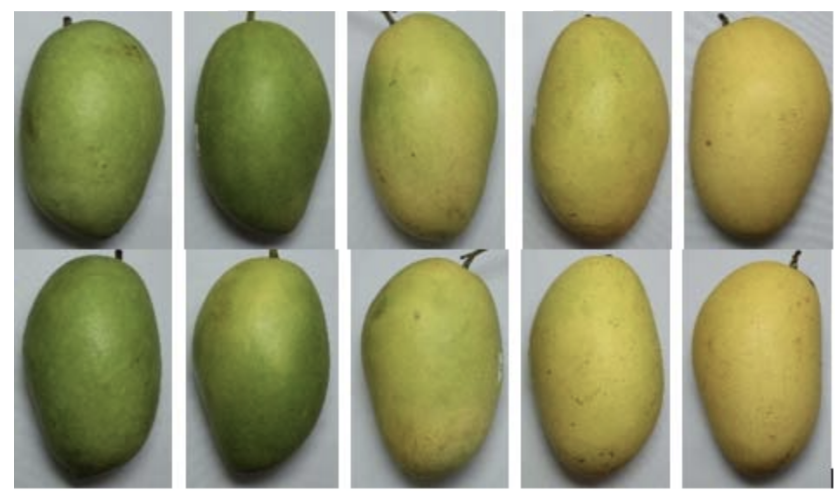
\includegraphics[width=0.5\textwidth]{fig1}
	\caption{Carabao Mangoes at Different Ripeness Stages \citep{guillermo-determining-2019}}
	\label{fig:img1}
\end{figure}
Carabao mangoes is a variety of a mango that is found and cultivated in the Philippines. It is known for its sweet signature taste that was recognized sweetest in the world in the Guinness Book of World Records in 1995. The mango was named after the national animal of the Philippines, a native breed of buffalo. On average, it is 12.5 cm in length and 8.5 cm in diameter, having a bright yellow color when ripe as seen in Figure 1.1. It is often cultivated during late May to early July \citep{DBpediaCarabao}.

As the Philippines is a tropical country, mangoes are a highly valued fruit as it is not only the country’s national fruit but also amongst the leading agricultural exports of the country, ranking only third below bananas and pineapples. This gives the country the 9th slot amongst the leading exporters of Mangoes across the world. Attributed to this ranking is the country's export of both fresh and dried mangoes, as well as low tariff rates. This allows the country to export a large quantity of the fruit in countries such as Singapore, Japan, and the USA as they can enter duty free markets provided by the World Trade Organization and Japan. Due to this, the mangoes have become a major source of income to an estimated 2.5 million farmers in the country \citep{centino-current-nodate}.

Before mangoes are sold in markets, they first undergo multiple post-harvest processes. This is to ensure that the mangoes that arrive in markets are utmost quality before being sold to consumers. Moreover, it ensures that mangoes are contained and preserved properly such that they do not incur damages and/or get spoiled on its transportation to the market. Processing of the mango involves pre-cooling, cleaning, waxing, classification, grading, ripening, packaging, preservation, storage, packing, and transportation \citep{patel-novel-2019} \citep{rizwan-iqbal-classification-2022}.

Among the processes that mangoes undergo, classification and grading is important as it allows the manufacturer to separate mangoes with good qualities versus mangoes with poor qualities. According to a study by \citep{lacap-bruise-2021}, size, length, width, volume, density, indention, and grooves are aspects that determine the maturity of mangoes. These traits are being checked along with the ripeness of the mango, sightings of bruise injury, and cracks on the fruit \citep{lacap-bruise-2021} as these aspects affect the sellability of the fruit as well as the chances of it getting spoiled sooner.

Previous studies have been made to automate the sortation process of the mangoes. Among these is a research done by \citet{abbas-mango-2018}, which focuses on classification of mangoes using their texture and shape features. They do this by, first, acquiring an image of the mango using a digital camera. Then, these images are fed to the MaZda package, which is a software originally developed for magnetic resonance imaging. Within the MaZda package is the B11 program, which uses Principal Component Analysis, Linear Discriminant Analysis, Nonlinear Discriminant Analysis, and texture classification to extract features from the mango, which in this case are the length, width, and texture. This data is then compared to a database in order to classify any given mango \citep{abbas-mango-2018}.  

Another study is done by \citet{rizwan-iqbal-classification-2022}, which classifies mangoes based on their color, volume, size, and shape This is done by making use of Charge Coupled Devices, Complementary Metal-Oxide Semiconductor sensors, and 3-layer Convolutional Neural Network. To classify the mangoes, images are first captured and preprocessed to be used as a data set \citep{rizwan-iqbal-classification-2022}. This data set is then augmented to be used as a model for the 3-layer Convolutional Neural Network. After extracting the features of the mango, the 3-layer Convolutional Neural Network is used as a method for their classification as it can mimic the human brain in pattern recognition, and process data for decision making. This is important as some mangoes have very subtle differences which make it difficult to differentiate them.



\section{Prior Studies}

A paper written by \citet{amna-et-al-machine-2023}, designed an automated fruit sorting machine based on the quality through 
an image acquisition system and CNN. Furthermore, the results of the paper show that the image processing detection 
score was 89\% while that of the tomatoes was 92\% while the CNN model had higher validity of 95\% for mangoes and 93\% 
for tomatoes. 15\%, while the percentage of distinction between the two groups was reported to be 5\% respectively 
\citep{amna-et-al-machine-2023}. Despite the high \gls{accuracy score}  in detecting mango defects, the fruit sorting system only sorts based 
on the mango defects and not on ripeness, and weight.

Furthermore, the research paper presented by \citet{guillergan-naive-2024} designed an Automated Carabao mango classifier, 
in which the mango image database is used to extract the features like size, area along with the ratio of the spots for 
grading using Naïve Bayes Model. For the results, the Naïve Bayes’ model recognized large and rejected mangoes with 95\%
 accuracy and the large and small/medium difference with a 7\% error, suggesting an application for quality differentiation 
 and sorting in the mango business industry. Despite the high accuracy of classifying Carabao mangoes, the researchers used a 
 high quality DSLR camera for the image acquisition system without any \gls{microcontroller} to control the mangoes \citep{guillergan-naive-2024}. 


\section{Problem Statement}
As mangoes are among the top exports of the Philippines \citep{centino-current-nodate}, 
assessing the physical deformities is a necessity. The physical deformities of the 
Carabao mango can determine the global competitiveness of the country. Having higher quality
 exports can often lead to gaining competitive edge, increase in demand, increase export revenues,
  and becoming less susceptible to low-wage competition \citep{dadamo-determinants-2018}. In order to increase the 
  quality of mango fruit exports, a key post-harvest process is done, which is sorting and grading.
   Mango sorting and grading then becomes important to determine which batches are of high quality and
    can be sold for a higher price, and which batches are of low quality and can only be sold for a low price
	 \citep{zhengzhou-first-industry-co-ltd-what-nodate}. Traditionally, fruit sorting and grading is inefficient as it is
	  done manually by hand. Some tools are used such as porous ruler to determine fruit size and color palette 
	  for color grading \citep{zhengzhou-first-industry-co-ltd-what-nodate}. However, among the problems encountered in the 
	  process of manually sorting and grading mangoes are susceptibility to human error and requiring a number of 
	  laborers to do the task. 

	  With the current advancements in technology, some researchers have already taken steps to automate the process
	   of sorting and grading mangoes. However, these attempts would often only consider some of the aspects 
	   pertaining to size, ripeness, and \gls{bruises} but not all of them at the same time. Lastly, not all research approaches
	    were able to implement a hardware for their algorithm, limiting their output to only a software implementation and not
		 an embedded system. As such the proposed system would assess the export quality of the Carabao mango based on all the
		  mentioned mango traits, namely size, \gls{bruises}, and ripeness while also taking into consideration being non-destructive.
		   These aspects are important because, as was previously mentioned, there is a need to develop a Carabao mango sorter 
		   that takes into account all these aspects at the same time while being non-destructive.



\section{Objectives and Deliverables}

\subsection{General Objective (GO)}
\begin{itemize}
	\item \Copy{GO}{GO: To develop a user-priority-based grading and sorting system for Carabao mangoes, 
 using machine learning and computer vision techniques to assess ripeness, size, and bruises. };
\end{itemize}

\subsection{Specific Objectives (SOs)}

\begin{itemize}
	\item \Copy{SO1}{SO1: To make an image acquisition system with a conveyor belt for 
	automatic sorting and grading mangoes. };
	
	\item \Copy{SO2}{SO2: To get the precision, recall, F1 score, confusion matrix,
	 and train and test accuracy metrics for classifying the ripeness and bruises with an accuracy score of at least 90\%.};
	
	\item \Copy{SO3}{SO3: To create a microcontroller-based system to operate the image acquisition system, 
	control the conveyor belt, and process the mango images through machine learning. };

	\item \Copy{SO4}{SO4: To grade mangoes based on user priorities for size, ripeness, and bruises.  };
	
	\item \Copy{SO5}{SO5: To classify mango ripeness based on image data using machine learning algorithms
	 such as kNN, k-mean, and Naïve Bayes.  };
	
	\item \Copy{SO6}{SO6: To classify mango size based on image data by getting its length and width using OpenCV, 
	geometry, and image processing techniques. };

	\item \Copy{SO7}{SO7: To classify mango bruises based on image data by employing machine learning algorithms.}
\end{itemize}

%\Copy{SO9}{To classify mango bruises based on image data by employing machine learning algorithms.}


\subsection{Expected Deliverables}

Table~\ref{tab:expd1} and ~\ref{tab:expd2} shows the outputs, 
products, results, achievements, gains, realizations, and/or
yields of the \documentType. 

\begin{table}[!htbp]
	\caption{Expected Deliverables per Objective} 	
	\label{tab:expd1} 
	{\centering \scriptsize
		\begin{tabular}{p{0.3\textwidth}|p{0.6\textwidth}}
			\hline 
			\hline 
			\textbf{Objectives} & 
			\textbf{Expected Deliverables}\\ 
			\hline 
%%			\endfirsthead
%			\multicolumn{2}{c}%
%			{\textit{Continued from previous page}} \\
%			\hline
%			\hline 
%			\textbf{Objectives} & 
%			\textbf{Expected Deliverables}\\ 
%			\hline 
%%			\endhead
%			\hline 
%			\multicolumn{2}{r}{\textit{Continued on next page}} \\ 
%%			\endfoot
%			\hline 
%%			\endlastfoot
%			\hline		
			\Paste{GO} &
			\begin{minipage}{0.55\textwidth}
				\vspace{10pt} 
				\begin{itemize}
					\item To develop a Carabao mango grading and sorting system 
					\item To grade Carabao mangoes into three categories based on ripeness, size, and 
					bruises of the Carabao mangoes using machine learning.
					\item To integrate sensors and actuators to control the conveyor belt and image acquisition system.
				\end{itemize}
			\end{minipage} \\ \hline

			\Paste{SO1} & 
			\begin{minipage}{0.55\textwidth}
				\vspace{10pt}
				\begin{itemize}
					\item To make an image acquisition system with a camera and LED light source.
					\item To build a flat belt conveyor for moving the mangoes.
				\end{itemize}
			\end{minipage} \\ \hline

			\Paste{SO2} & 
			\begin{minipage}{0.55\textwidth}
				\vspace{10pt}
				\begin{itemize}
					\item To use a publicly available dataset of at least 10,000 mango images
					 for classification of ripeness, and bruises.
				\end{itemize}
			\end{minipage} \\ \hline
						
			\Paste{SO3} & 
			\begin{minipage}{0.55\textwidth}
				\vspace{10pt}
				\begin{itemize}
					\item To develop an intuitive UI where users can start and stop the system.
					\item To implement a priority-based grading system with sliders for ripeness, bruises, and size.
				\end{itemize}
			\end{minipage} \\ \hline
						
			\Paste{SO4} & 
			\begin{minipage}{0.55\textwidth}
				\vspace{10pt}
				\begin{itemize}
					\item To utilize a linear combination formula as the overall mango score, where each classification level 
					contributes a grade, weighted by the priority assigned to the three properties.
					\item To assign score values for each classification level of the mango.
				\end{itemize}
			\end{minipage} \\ \hline
		

			\Paste{SO5} & 
			\begin{minipage}{0.55\textwidth}
				\vspace{10pt}
				\begin{itemize}
					\item To train a machine learning model such as kNN, k-mean, naive Bayes capable
					of classifying mango ripeness based on the image color
					\item To gather a dataset of annotated images with ripeness labels
					\item To obtain an evaluation report of performance metrics of the model
				\end{itemize}
			\end{minipage} \\ \hline

			
		\end{tabular}	
			
	}
\end{table}


\begin{table}[!htbp]
	\caption{Expected Deliverables per Objective continued} 	
	\label{tab:expd2} 
	{\centering \scriptsize
		\begin{tabular}{p{0.3\textwidth}|p{0.6\textwidth}}
			\hline 
			\hline 
			\textbf{Objectives} & 
			\textbf{Expected Deliverables}\\ 
			\hline 
			\Paste{SO6} & 
			\begin{minipage}{0.55\textwidth}
				\vspace{10pt}
				\begin{itemize}
					\item To develop an image processing algorithm capable of determining mango 
					size using OpenCV, NumPy, and imutils
					\item To classify mangoes based on size and categories into small, medium, 
					and large based on those measures
				\end{itemize}
			\end{minipage} \\ \hline

			\Paste{SO7} & 
			\begin{minipage}{0.55\textwidth}
				\vspace{10pt}
				\begin{itemize}
					\item To train a machine learning model such as 
					CNN capable of distinguishing bruised and non-bruised mangoes
					\item To train a machine learning model such as kNN, k-mean, and Naïve Bayes 
					capable of assessing the extent of bruising on the mangoes if it is significant or partial
					\item To gather a dataset of annotated images based on bruises
					\item To obtain an evaluation report of performance metrics of both CNN and machine learning models
				\end{itemize}
			\end{minipage} \\ \hline
		\end{tabular}
	}
\end{table}


% \begin{center}
% 	{\scriptsize
% 		\begin{longtable}{p{0.2\textwidth}|p{0.6\textwidth}|p{0.1\textwidth}}
% 			\caption{Summary of methods for reaching the objectives} \label{tab:methods_per_objective} \\
% 			\hline 
% 			\hline 
% 			\textbf{Objectives} & 
% 			\textbf{Expected Deliverables} &
% 			\textbf{Locations}\\ 
% 			\hline 
% 			\endhead
% 			\hline 
% 			\multicolumn{3}{r}{\textit{Continued on next page}} \\ 
% 			\endfoot
% 			\hline 
% 			\endlastfoot
% 			\hline
% 			\Paste{GO} & \begin{itemize}
% 				\item To develop a Carabao mango grading and sorting system 
% 				\item To grade Carabao mangoes into three categories based on ripeness, size, and 
% 				bruises of the Carabao mangoes using machine learning.
% 				\item To integrate sensors and actuators to control the conveyor belt and image acquisition system.
% 			\end{itemize} & Sec.~\ref{sec:implement} on p.~\pageref{sec:implement}\\ \hline
			
% 			\Paste{SO1} & \begin{itemize}
% 				\item To make an image acquisition system with a camera and LED light source.
% 				\item To build a flat belt conveyor for moving the mangoes.
% 			\end{itemize} & Sec.~\ref{sec:implement} on p.~\pageref{sec:implement} \\ \hline
			
% 			\Paste{SO2} & \begin{itemize}
% 				\item To use a publicly available dataset of at least 10,000 mango images
% 				 for classification of ripeness, and bruises.
% 			\end{itemize} & Sec.~\ref{sec:implement} on p.~\pageref{sec:implement}\\ \hline
			
% 			\Paste{SO3} & \begin{itemize}
% 				\item To develop an intuitive UI where users can start and stop the system.
% 				\item To implement a priority-based grading system with sliders for ripeness, bruises, and size.
% 			\end{itemize} & Sec.~\ref{sec:implement} on p.~\pageref{sec:implement}\\ \hline
			
% 			\Paste{SO4} & \begin{itemize}
% 				\item To utilize a linear combination formula as the overall mango score, where each classification level 
% 				contributes a grade, weighted by the priority assigned to the three properties.
% 				\item To assign score values for each classification level of the mango.
% 			\end{itemize} & Sec.~\ref{sec:implement} on p.~\pageref{sec:implement} \\ \hline
			
% 			\Paste{SO5} & \begin{itemize}
% 				\item To train a machine learning model such as kNN, k-mean, naive Bayes capable
% 				of classifying mango ripeness based on the image color
% 				\item To gather a dataset of annotated images with ripeness labels
% 				\item To obtain an evaluation report of performance metrics of the model
% 			\end{itemize} & Sec.~\ref{sec:implement} on p.~\pageref{sec:implement} \\ \hline

% 			\Paste{SO6} & \begin{itemize}
% 				\item To develop an image processing algorithm capable of determining mango 
% 				size using OpenCV, NumPy, and imutils
% 				\item To classify mangoes based on size and categories into small, medium, 
% 				and large based on those measures
% 			\end{itemize} & Sec.~\ref{sec:implement} on p.~\pageref{sec:implement} \\ \hline

% 			\Paste{SO7} & \begin{itemize}
% 				\item To train a machine learning model such as 
% 				CNN capable of distinguishing bruised and non-bruised mangoes
% 				\item To train a machine learning model such as kNN, k-mean, and Naïve Bayes 
% 				capable of assessing the extent of bruising on the mangoes if it is significant or partial
% 				\item To gather a dataset of annotated images based on bruises
% 				\item To obtain an evaluation report of performance metrics of both CNN and machine learning models
% 			\end{itemize} & Sec.~\ref{sec:implement} on p.~\pageref{sec:implement} \\ \hline
			
% 		\end{longtable}
% 	}
% \end{center}

\section{Significance of the Study}

Automating the process of sorting and grading mangoes increases efficiency and 
productivity for the user which would in effect remove human error in sorting and
 grading and decrease the human labor and time taken to sort and grade the mangoes.
  This is especially important for farmers with a large amount of fruit such as mangoes and a
   lesser labor force. A recent study showed that
    their automated citrus sorter and grader using computer vision can reduce the human
	 labor cost and time to sort and grade when comparing the automated citrus sorter and grader
	  to manual human labor \cite{chakraborty-development-2023}. 

Another benefit to automating sorting and grading mangoes is the improvement in quality control.
 This implies that compared to human labor, automating sorting and grading mangoes can uniformly 
 assess the quality of mangoes based on size, color, and \gls{bruises}, ensuring that the expected grade and high-quality mangoes reach the consumer. By accurately identifying substandard mangoes, the system 
  helps in reducing waste and ensuring that only marketable fruits are processed further.

Likewise, the scalability of automating sorting and grading mangoes is simpler, especially 
for lower labor force farmers with large volumes of mangoes. Because of the possibility of
 large-scale operations by automating sorting and grading mangoes, farmers can now handle large
  volumes of mangoes, making them suitable for commercial farms and processing plants. Moreover,
   it can be adapted to different varieties of mangoes and potentially other fruits with minor modifications.


\subsection{Technical Benefit}

\begin{enumerate}
	\item The development of an automated \gls{Carabao mango} sorter would increase the quality control 
	of classifying \gls{Carabao mango} based on ripeness, size, and bruising.
	
	\item The accuracy in sorting Carabao mangoes will be significantly improved while
	 reducing the errors due to human factors in manual sorting.
	
	\item The automated \gls{Carabao mango}  sorter carefully sorts the mangoes 
	while ensuring that they remain free from bruising or further damage during the process	
\end{enumerate}

\subsection{Social Impact}

\begin{enumerate}
	\item The reduction in manual labor creates opportunities in maintenance and
	 technologies in the automated \gls{Carabao mango}  sorter.
	
	\item The automated \gls{Carabao mango}  sorter system improves Carabao mango 
	standards and enhances the satisfaction of the buyers and the customers through
	 guaranteeing consistent Carabao mango grade.
	
	\item Opportunity to increase sales and profit for the farmers through consistent 
	quality and grade Carabao mangoes while reducing the physical labor to sort it.
\end{enumerate}

\subsection{Environmental Welfare}

\begin{enumerate}
	\item With the utilization of non-destruction methods of classifying Carabao mangoes together with an
	 accurate sorting system, overall waste from Carabao mangoes is reduced and the likelihood
	  of improperly sorted mangoes is decreased.
	
	\item Automation of sorting and grading Carabao mangoes promotes sustainable farming practices.
	
\end{enumerate}



\section{Assumptions, Scope, and Delimitations}

\subsection{Assumptions}

\begin{enumerate}
	\item The Carabao mangoes are from the same source together with the same variation
	
	\item The Carabao mangoes do not have any fruit borer and diseases
	
	\item All the components do not have any form of defects
	\item The prototype would have access to constant electricity/power source.
	\item The Carabao mangoes to be tested would be in the post-harvesting stage and in the grading stage.
	\item The image-capturing system would only capture the two sides of the mango which 
	are the two largest surface areas of the skin.	
\end{enumerate}

\subsection{Scope}
\begin{enumerate}
	\item The prototype would be specifically designed to grade and 
	sort Carabao Mangoes based on only ripeness, size, and visible skin bruises.
	
	\item The mangoes used as the subject will be solely sourced from markets in the Philippines.
	
	\item The Carabao mangoes would be graded into three levels.
	\item The prototype will be using a microcontroller-based system locally stored on 
	the device itself to handle user interaction.
	\item Computer vision algorithms to be used will include image classification.
\end{enumerate}

\subsection{Delimitations}
\begin{enumerate}
	\item The project would only be able to perform sorting and grading on one specific fruit 
	which is the Carabao mango and will not be able to sort other types of mangoes.
	
	\item Additionally, the project prototype will only be able to capture, sort, and grade one 
	mango subject at a time which means the mangoes have to be placed in the conveyor belt in
	 a single file line for accurate sorting. 
	
	\item For the bruises, the system will only be able to detect external bruises and 
	may not identify the non-visible and internal bruises.
	\item The system does not load the mangoes onto the conveyor belt itself. 
	Assistance is required to put mangoes into the conveyor belt to start the sorting process
	\item The prototype will be powered using \acr{ac} power and will be plugged into 
	a wall socket which is only suitable for indoor use.
\end{enumerate}

\section{Description and Methodology of the \documentType}

A purpose of the description here is to re-steer/remind the panelist/reader again by tersely describing what your thesis is about (i.e. the problem and the main goal you want to achieve) in another way without sounding repetitive. 

Your methodology is your means of achieving your stated objectives. What you put here is the summary of your methodology chapter.



\graytx{\blindtext}


\ifFinished
\else

\section{Estimated Work Schedule and Budget}

\begin{figure}[!htbp]
	\centering
	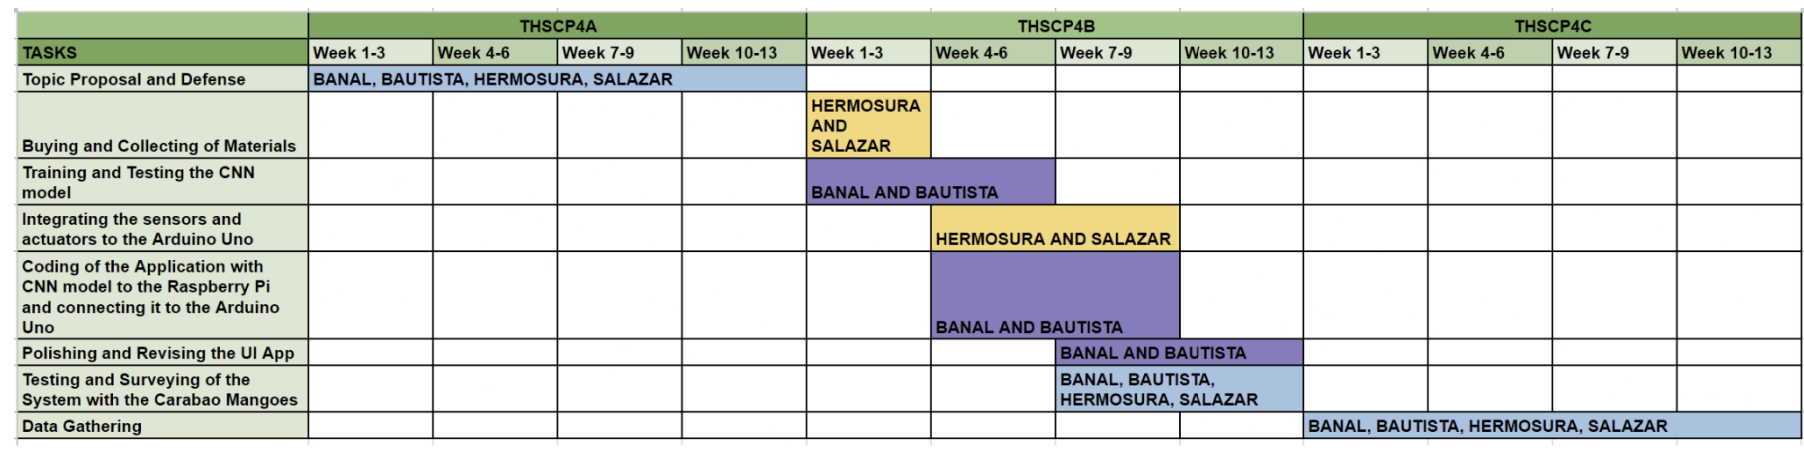
\includegraphics[width=1\textwidth]{ganttchart}
	\caption{Gantt Chart}
	\label{fig:img2}
\end{figure}

As seen above, Table~\ref{fig:img2} shows the Gantt Chart together with the assigned task. For the
first part of the THSCP4A, the group would primarily revise and fine tune Chapters 1
and 2 while also preparing for the defense. After that for THSCP4B, the yellow team
which consists of two members, Hermosura and Salazar, would start buying and
collecting the materials needed for assembling the prototype. While team yellow is
doing that, team purple which consists of Banal and Baustista would start training and
validating the \acr{cnn} model based on the Carabao mango image dataset. After that
integration of the sensors and actuators together with the integration of the \acr{cnn} model
and beginning of coding of the Application to the Raspberry Pi would be done. Once
that \acr{cnn} model is deployed and the Application works testing of the Carabao mangoes
to the prototype would be done. During THSCP4C, data gathering would be done
together with polishing and revising of the final paper.

\ifPhD
\section{Publication Plan}
\graytx{\blindtext}
\fi

\fi


\section{Overview of the \documentType}

There are seven succeeding chapters. To recall, chapter 1 involves the introduction of the
thesis topic containing the background of the study, previous studies, objectives and
deliverables, assumptions, scope, and delimitation, significance of the study, description
of the project together with the methodology, and Gantt chart and budget. Chapter 2
involves the existing articles, the lacking in their approaches, and the summary of
chapter 2. Chapter 3 involves the theoretical considerations of the thesis topic while
chapter 4 would consist of the design consideration involving the thesis topic. Chapter 5
would involve the research methodology containing the testing procedure and setup.
Chapter 6 would involve the results and discussion based on the methodology while
Chapter 7 would involve the conclusion, recommendations, and future suggestions.

	%\stopcontents[chapters]
	\cleardoublepage
	
	%%%%%%%%%%%%%%%%%%%%%%%%%%%%%%%%%%%%%%%%%%%%%%%%
	\chapter{Literature Review} 
	\label{ch:litrev} 
	%\startcontents[chapters]
	%\begin{SingleSpace}	
	%	\Mprintcontents 
	%\end{SingleSpace}
	

\section{Existing Work}

The research paper written by Adam et. al. (2022) developed a ripeness grader for
Carabao mangoes. The Carabao mango ripeness grade calculated based on object and
color detection which were written in microcontroller. These are the systems designed
by the researchers that consists of Raspberry Pi 4, Arduino Uno, camera, touch screen
LCD, MQ3 gas sensor, ventilation system. The proposed system was able to ascertain an
overall reliability of 95\%: therefore, the specified objective of ascertaining the ripeness
level of the mangoes was met with success. However, accuracy and reliability of the
software system are there since the hardware design does not seem to be workable when
one must deal with the scores of mangoes \cite{adam-non-destructive-2022}. In addition, the design of the hardware does
not integrate any form of physical automating, say like the conveyor belt. Besides, the
hardware system only works efficiently when deciding the ripeness grade of mangoes
separately.

A study done by Samaniego et. al. (2023) is another research paper that supports and has
relevant information concerning the topic. The researchers proposed a fully-perovskite
photonic system which has the capability to identify and sort or grade mango based on
features such as color, weight and, conversely, signs of damages \cite{school-of-engineering-asia-pacific-college-philippines-carabao-2023}. Some of the techniques
in image processing that the researchers used included image enhancement, image
deblurring, edge detection using MATLAB and Arduino as well as color image
segmentation. By carrying out the multiple trials on the device they achieved a
classification speed of 8.132 seconds and an accuracy of 91.2\%. The proponents’
metrics used for the ratings were speed wherein the results were rated “excellent” while
the accuracy rating given was “good”. One of the limitations of the paper is that the
researchers were only limited to the color, texture, and size of the Carabao mango

Furthermore, the research paper presented by Guillergan et. al. (2024) designed an
Automated Carabao mango classifier, in which the mango image database is used to
extract the features like weight, size, area along with the ratio of the spots for grading
using Naïve Bayes Model. Concerning the quantitative test design, one had to control
and experiment with various methods of image processing that would improve the
likelihood of improved classification. The paper methodology entailed sample collection
from 300 Carabao mangoes, picture taking using a DSLR camera, and feature
deconstruction for categorization \cite{guillergan-naive-2024}. The system prototype and
the software were designed with the programming language C\# with integration of
Aforge. NET routines. The performance of this model was checked with the help of the
dataset containing 250 images, precision, recall, F-score key indicators were used. The
investigation discovered that the Naïve Bayes’ model recognized large and rejected
mangoes with 95\% accuracy and the large and small/medium difference with a 7\% error,
suggesting an application for quality differentiation and sorting in the mango business
industry. The limitations in the researchers’ paper include the researchers were able to
achieve high accuracy after using a high quality DSLR camera and the fact that the
researchers were not able to incorporate the use of microcontrollers.

\begin{table}[h]
	\centering
	\caption{Comparison of Existing Studies}
	\label{tab:comparison_existing_studies}
	\renewcommand{\arraystretch}{1.3}
	\begin{tabular}{p{0.2\textwidth}|p{0.6\textwidth}|p{0.1\textwidth}}
		\hline
		\textbf{Existing Study} & \textbf{Limitations} & \textbf{Accuracy Rating} \\
		\hline
		\cite{adam-non-destructive-2022} & No physical automation, not suitable for large amounts of mangoes, only classifies ripeness and only a sample size of 10 mangoes. & 95\% \\
		\hline
		\cite{school-of-engineering-asia-pacific-college-philippines-carabao-2023} & Focuses only on color and size. & 91.2\% \\
		\hline
		\cite{guillergan-naive-2024} & Relies on high-quality DSLR cameras, and limited automation due to not integrating microcontrollers. & 95\% \\
		\hline
		\cite{supekar-multi-parameter-2020} & No physical automation implemented. Ripeness, size, and shape-based classification achieved 100\%, 98.19\%, and 99.20\% accuracy respectively on their own. However, errors occurred when taking into account all these aspects together for grading mangoes, causing an accuracy rating deduction. & 88.88\% \\
		\hline
	\end{tabular}
\end{table}

Previous studies on mango grading have achieved an accuracy rating of up to 95\%, as
shown in Table~\ref{tab:comparison_existing_studies}. However, these studies either relied on a small sample size, which
limits statistical significance, or utilized expensive equipment, which may be
impractical. In light of this, the researchers have set a target accuracy rating of greater than or equal to 90\%.
This target ensures that the system being developed is comparable to, or better than,
existing studies that used larger sample sizes or assessed multiple mango traits at the
same time. Furthermore, this research aims to distinguish itself by not only maintaining
or exceeding the 90\% accuracy rating but also incorporating a graphical user interface
(GUI) for selective priority-based mango classification. The system will integrate both
software and hardware components, and it will evaluate a greater number of mango
traits for grading purposes.

\subsection{Sorting Algorithms}
In previous studies, researchers have implemented various artificial intelligence
algorithms in order to determine the optimal and most effective method for sorting
mangoes. One of the algorithms that was used in the classification of mangoes was the
CNN or Convolutional Neural Networks. A study done by Zheng and Huang (2021)
explored the effectiveness of CNN, specifically in classifying mangoes through image
processing. The system that the researchers developed graded mangoes into four groups
which was based on the Chinese National Standard \cite{zheng-mango-2021}. These mangoes were examined by
their shape, color uniformity, and external defects. The system that was developed had
an impressive accuracy of 97.37\% in correctly classifying the mangoes into these
grading categories
Support Vector Machine was also one of the classification algorithms that was
implemented to detect flaws in mangoes. In that study by Veling (2019), SVM
was used in the classification of diseases from mangoes. The study used 4 different
diseases/defects for testing \cite{veling-mango-2019}. The diseases were Anthracnose, Powdery Mildew, Black
Banded, and Red Rust. and provided 90\% accuracy for both the leaves and the fruit

In the study done by Schulze et. al. (2015), Simple
Linear Regression, Multiple Linear Regression, and Artificial Neural Network models
were all studied and compared for the purpose of size-mass estimation for mango fruits.
The researchers found that the Artificial Neural Network yielded a high accuracy rating
for mass estimation and for mango classification based on size with a success rate of
96.7\% \cite{schulze-development-2015}. This is attributed to the Artificial Neural Network model’s ability to learn both
linear and nonlinear relationships between the inputs and the outputs. However, a
problem can occur with the use of the model, which is overfitting. This issue occurs
when the model is overtrained with the data set such that it will start to recognize
unnecessary details such as image noise which results in poor generalization when fed
with new data. With this in mind, additional steps will be necessary to mitigate the issue.
Another research article written by Alejandro et. al. (2018)
implements a method for sorting and grading Carabao mangoes. This research focuses
on the use of Probabilistic Neural Network, which is another algorithm that is used for
pattern recognition and classification of objects. For this study, the researchers focused
on the area, color, and the black spots of the mango for their Probabilistic Neural
Network model \cite{alejandro-grading-2018}. Their research using the model yielded an accuracy rating of 87.5\% for
classification of the mangoes which means it is quite accurate for classifying mangoes
within the predefined categories. However, problems were encountered with the use of
the model when trying to identify mangoes that did not fit the predefined size categories
of small, medium, and large. This means that the PNN model may become challenged
when presented with a mango with outlying traits or traits that were very different from
the data set.

\begin{table}[h]
	\centering
	\caption{Comparison of Sorting Algorithm Models}
	\label{tab:sorting_algorithm_models}
	\renewcommand{\arraystretch}{1.3} % Adjust row spacing
	\begin{tabular}{p{0.3\textwidth}|p{0.1\textwidth}|p{0.2\textwidth}|p{0.3\textwidth}}
		\hline
		\textbf{Sorting Algorithm Model} & \textbf{Accuracy Rating} & \textbf{Criteria} & \textbf{Problems Encountered} \\
		\hline
		Convolution Neural Network & 97.37\% & shape, color, defects & Minor blemishes affected the accuracy. \\
		\hline
		Support Vector Machine & 90\% & mango defects and diseases & The model is sensitive to noise, which requires intensive image preprocessing. \\
		\hline
		Artificial Neural Network & 96.7\% & for mango size and mass & Overfitting \\
		\hline
		Probabilistic Neural Network & 87.5\% & for mango area, color, and black spots & Difficulty in identifying mangoes that have outlying features or did not fit the predefined 		categories \\
		\hline
	\end{tabular}
\end{table}

\section{Lacking in the Approaches}
%todo put the citations correctly
The majority of past researchers such as Amna et. al. (2023) and Guillergan et. al.
(2024) were able to implement a fruit and mango sorter together with an accurate AI
algorithm to detect the ripeness defects. This means that none of the previous research
papers were able to integrate an interchangeable user-priority-based grading together
with size, ripeness, and bruises using machine learning for Carabao mango sorter and
grader. Our research however would implement an automated Carabao mango sorter in
terms of size, ripeness, and bruises with its own UI, conveyor belt, stepper motors, and
bins for collecting the different ripeness and defect grade of the Carabao mango.

\section{Summary}
%todo put the citations correctly
To reiterate, there is an innovative gap that needs to be filled with regards to the process
of sorting and grading Carabao mangoes. The traditional methods for conducting this
process manually by hand, by a porous ruler, by a sugar meter, and by a color palette can
be prone to human error and expensive costs due to the number of laborers required to
do the task. On the other hand, although researchers have already taken steps to
automate the process of mango sorting and grading, there is still a need for an
implementation that takes into account size, ripeness, and bruises altogether whilst being
non-destructive and having its own embedded system. The research articles shown
above show the different computer vision and CNN approaches for sorting and
classifying mangoes. For example, a system created by Adam et al. (2022) was more
focused on ripeness detection. Samaniego et al. (2023) considered photonic systems for
grading mango fruit based on color and weight. On the other hand, Guillergan et al.
(2024) implemented the Naïve Bayes classification model on mangoes with high
accuracy, which thereby did not include any microcontroller. There was an attempt to
study each of those parameters separately and that is why the multifactorial approach
was not used. With this in mind, the system being proposed does exactly what was
mentioned, to implement a non-destructive and automated sorting and grading system
for Carabao mangoes that takes into account size, ripeness, and bruises altogether using
machine learning, as well as having its own embedded system. This system will be
mainly composed of a conveyor belt, servo motors, a camera, microcontrollers, and an
LCD display for the user interface. By doing so, the system should be able to improve
the efficiency and productivity of mango sorting and grading, remove the effect of
human error and reduce time consumption. The studies also provided critical insights
regarding the effective algorithms that can be used in classification stages in image
processing. The use of CNN had the most accuracy with manageable potential
challenges. Lastly, by scaling the implementation, the overall export quality of the
Carabao mangoes can be improved.





	%\stopcontents[chapters]
	\cleardoublepage
	
	%%%%%%%%%%%%%%%%%%%%%%%%%%%%%%%%%%%%%%%%%%%%%%%%
	\chapter{Theoretical Considerations}
	%\chaptermark{Theoretical Considerations} % uncomment this and put a shorter version of the chapter title for the TOC and chapter markings (i.e., header or footer)
	\label{ch:theorycon}
	%\startcontents[chapters]
	%\begin{SingleSpace}	
	%	\Mprintcontents 
	%\end{SingleSpace}
	
%This chapter is for providing the context to your panelist/reader.  It is actually an expanded form of the Background of the Study that you have put in Chapter~\ref{ch:intro}.

To start, computer vision plays an important and pivotal role in machine learning as it equips machines and other systems with the ability to perceive, interpret and understand visual information from our physical environment. Equipping computer systems with this human-like vision capability can be very helpful in many applications such as autonomous driving, advanced medical image analysis and many more. One of the most basic yet very critical functions of computer vision is to process and analyze images to detect and classify objects. This is one of the most important attributes of vision as it can be very useful once computers can correctly recognize and identify different objects. This is where machine learning algorithms further improve its significance. As these computer vision models are exposed to more visual data and information, it can improve in terms of its accuracy and correctness when it comes to identifications and even predictions. This adaptability can be very critical on the performance of these machine vision models in different settings with different lighting conditions which can effectively alter image quality.  

\begin{figure}[!htbp]
	\centering
		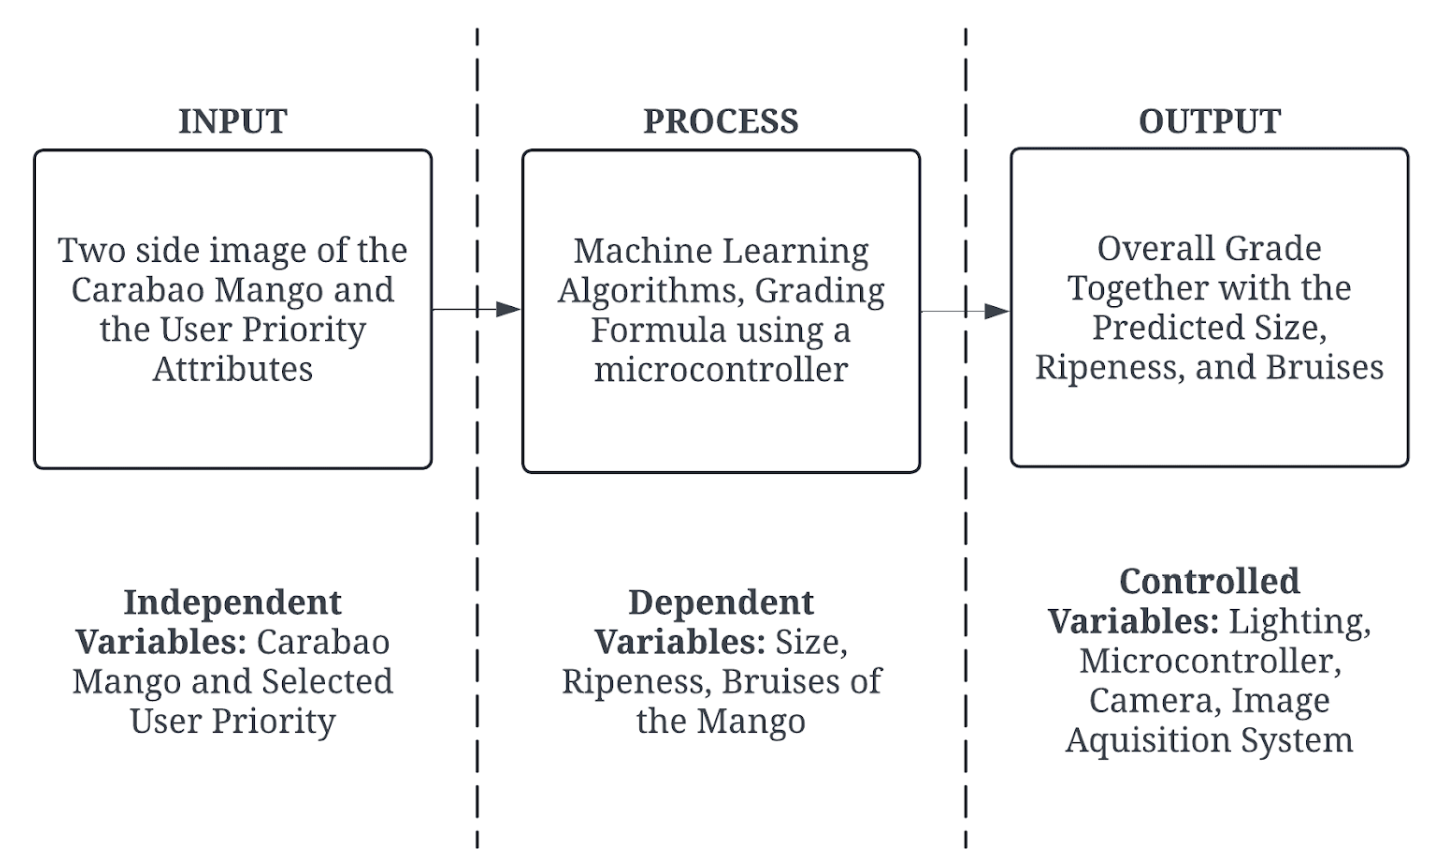
\includegraphics[width=0.9\textwidth]{conceptdiagram}
	\caption{Conceptual Framework }
	\label{fig:conceptdiagram}
\end{figure}

\section{Summary}

Provide the gist of this chapter such that it reflects the contents and the message.
	%\stopcontents[chapters]
	\cleardoublepage
	
	%%%%%%%%%%%%%%%%%%%%%%%%%%%%%%%%%%%%%%%%%%%%%%%%
	\chapter{Design Considerations} 
	\label{ch:designcon} 
	%\startcontents[chapters]
	%\begin{SingleSpace}	
	%	\Mprintcontents 
	%\end{SingleSpace}
	
Likewise, the objective of chapter 4 is to describe the researcher's design 
consideration when developing and testing the prototype. For an overview of 
the design of the prototype, the researchers considered different computer vision models in
 classifying the ripeness and bruises together with other algorithms to determine 
 the size of the mango. Likewise, the hardware design was also taken into consideration where 
 the physical design of the conveyor belt was taken into account.

\section{Introduction}
This chapter discusses the design considerations for the mango 
sorting and grading system, focusing on the technical and engineering decisions 
required for its development. The design process aims to create a scalable, efficient, 
and user-friendly system that leverages machine learning for accurate mango classification.

\section{System Architecture}
The system architecture is represented through a block diagram, showcasing modules such as image acquisition, 
preprocessing, feature extraction, machine learning model, and grading output. Each module is described in detail, 
emphasizing its role in the overall system. For instance, the image acquisition module uses high-resolution cameras 
to capture mango images, while the preprocessing module enhances image quality for better feature extraction.

\section{Hardware Considerations}
The hardware components include high-resolution cameras, lighting systems for consistent image capture, and 
microcontrollers like Raspberry Pi or Arduino for system control, actuators like DC and stepper motors to move 
the mangoes. The choice of hardware is justified based on cost, performance, and compatibility with the software framework.

\subsection{General Prototype Framework}
\begin{figure}[!htbp]
	\centering
	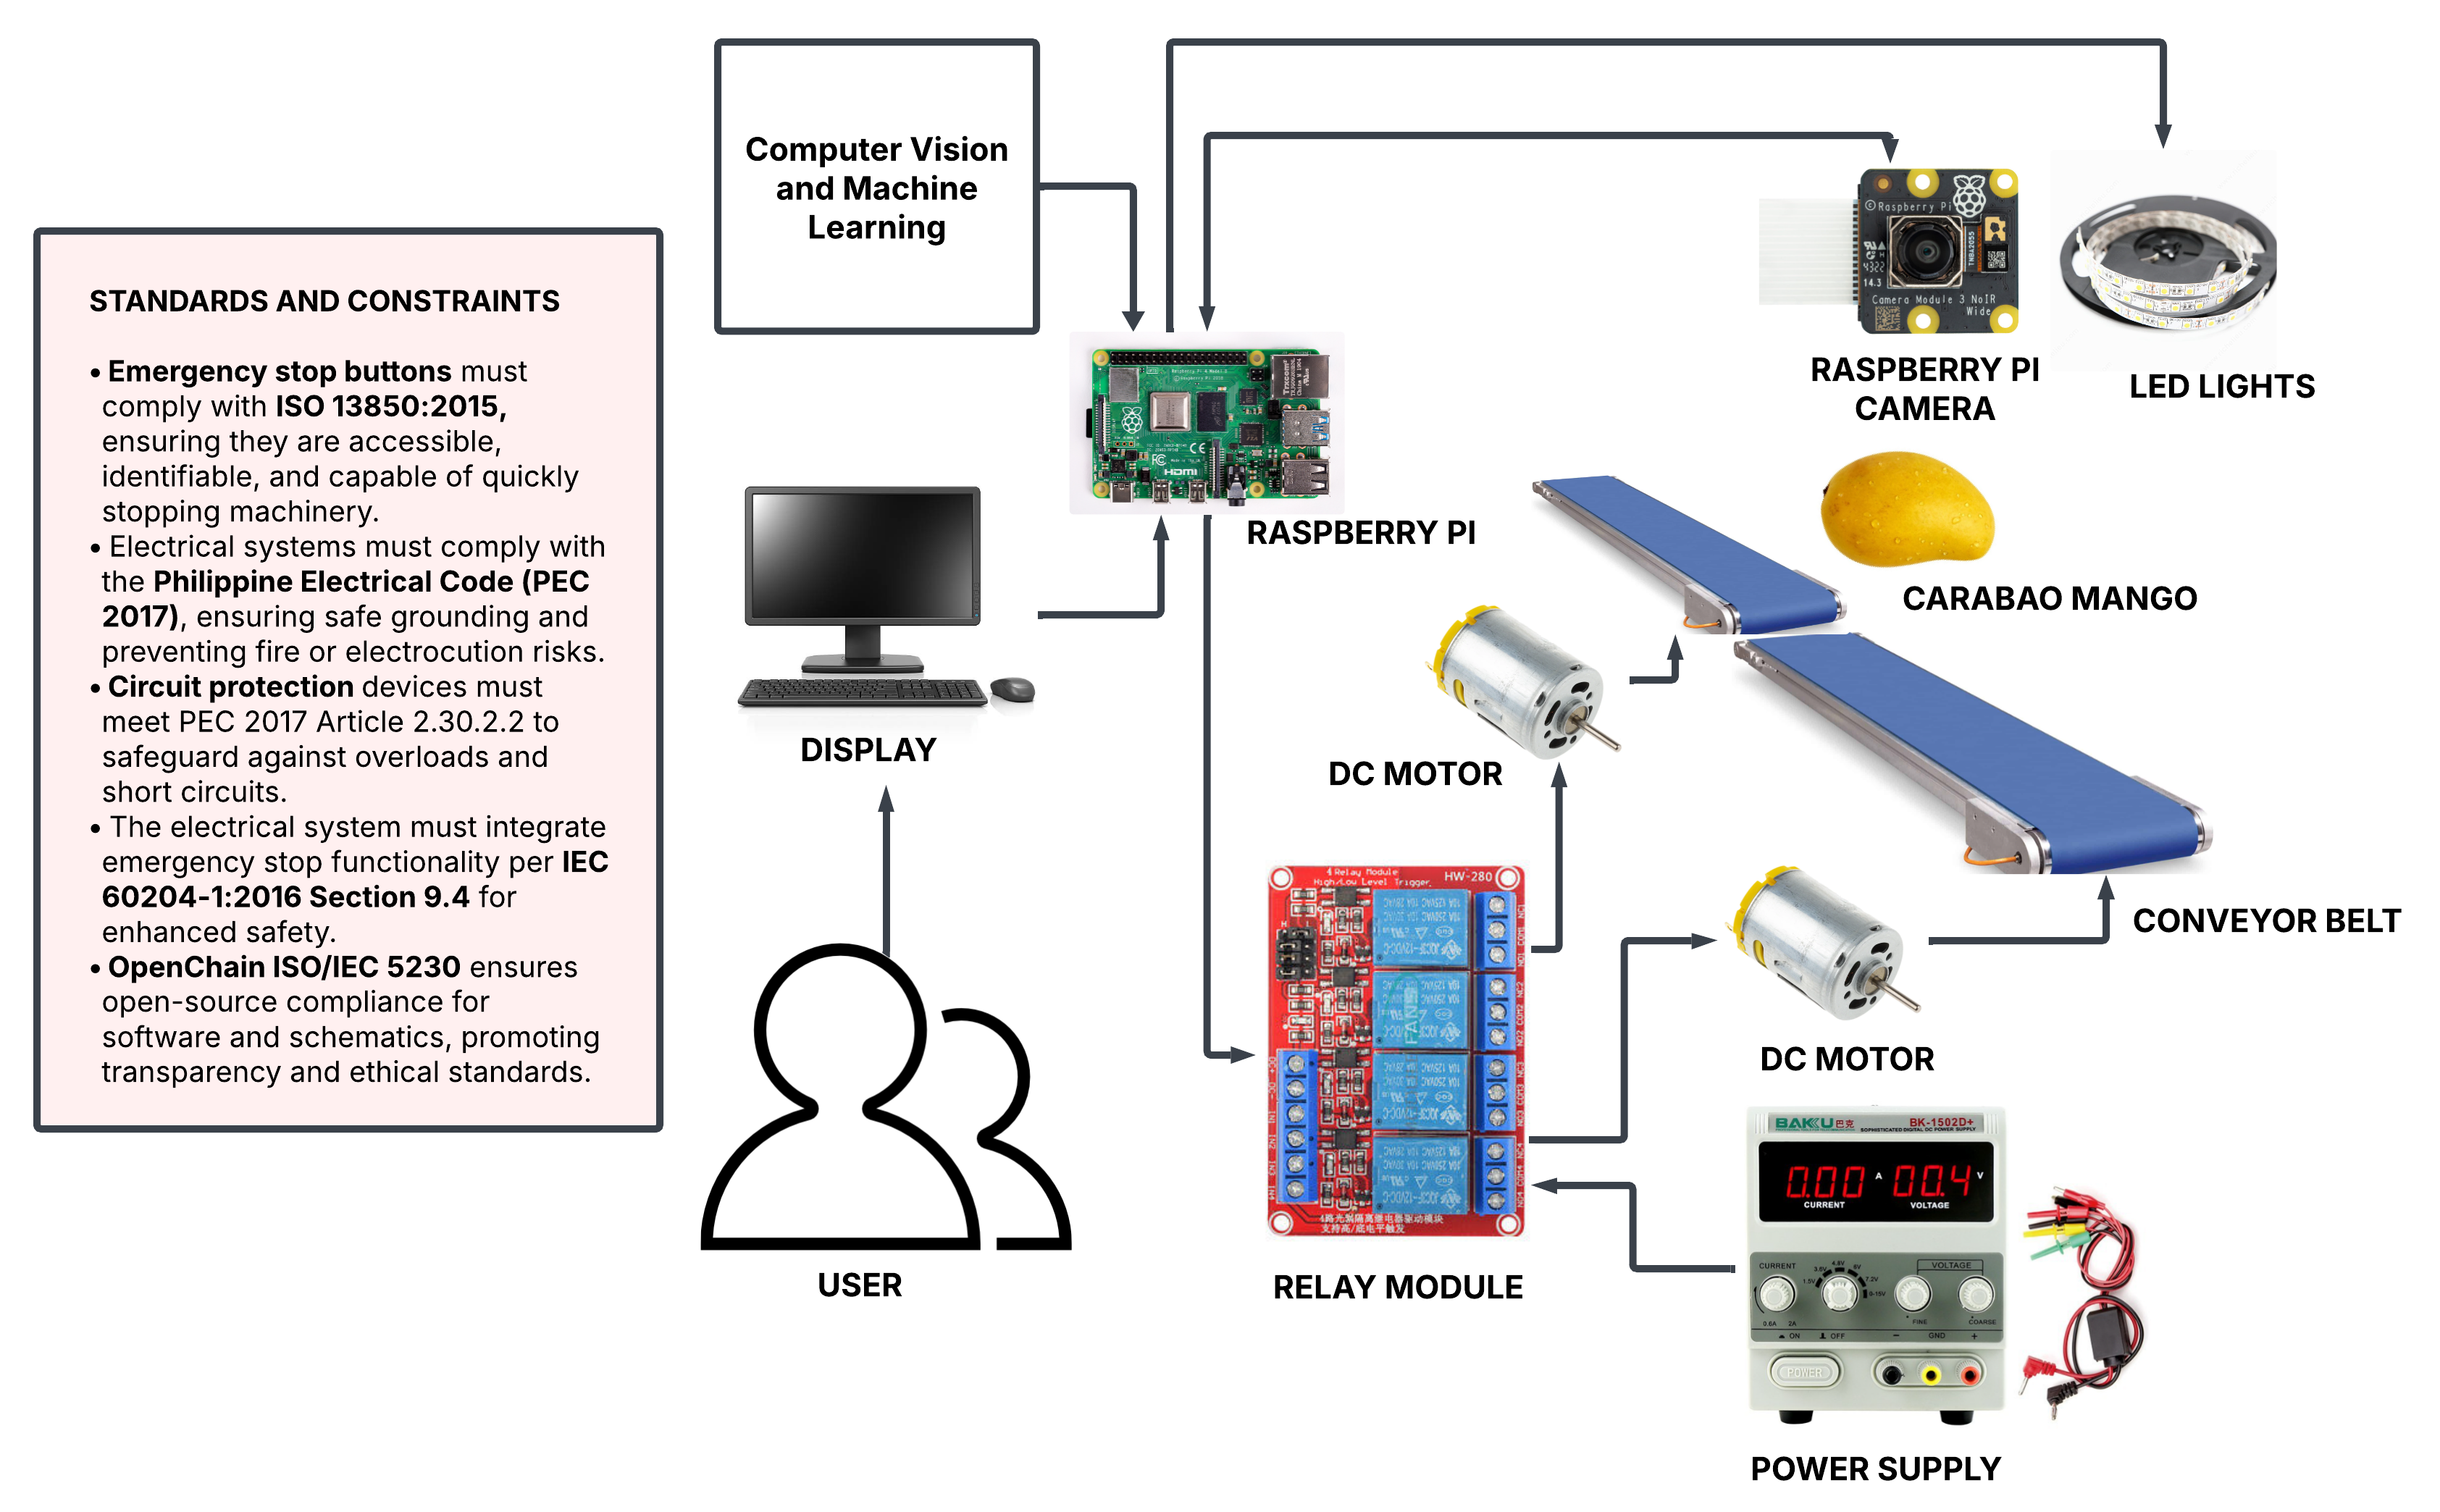
\includegraphics[width=0.9\textwidth]{pro2typediagram}
	\caption{Prototype Framework}
	\label{fig:prototypeDiagram_fig}
\end{figure}

\subsection{Prototype Flowchart}
\begin{figure}[!htbp]
	\centering
	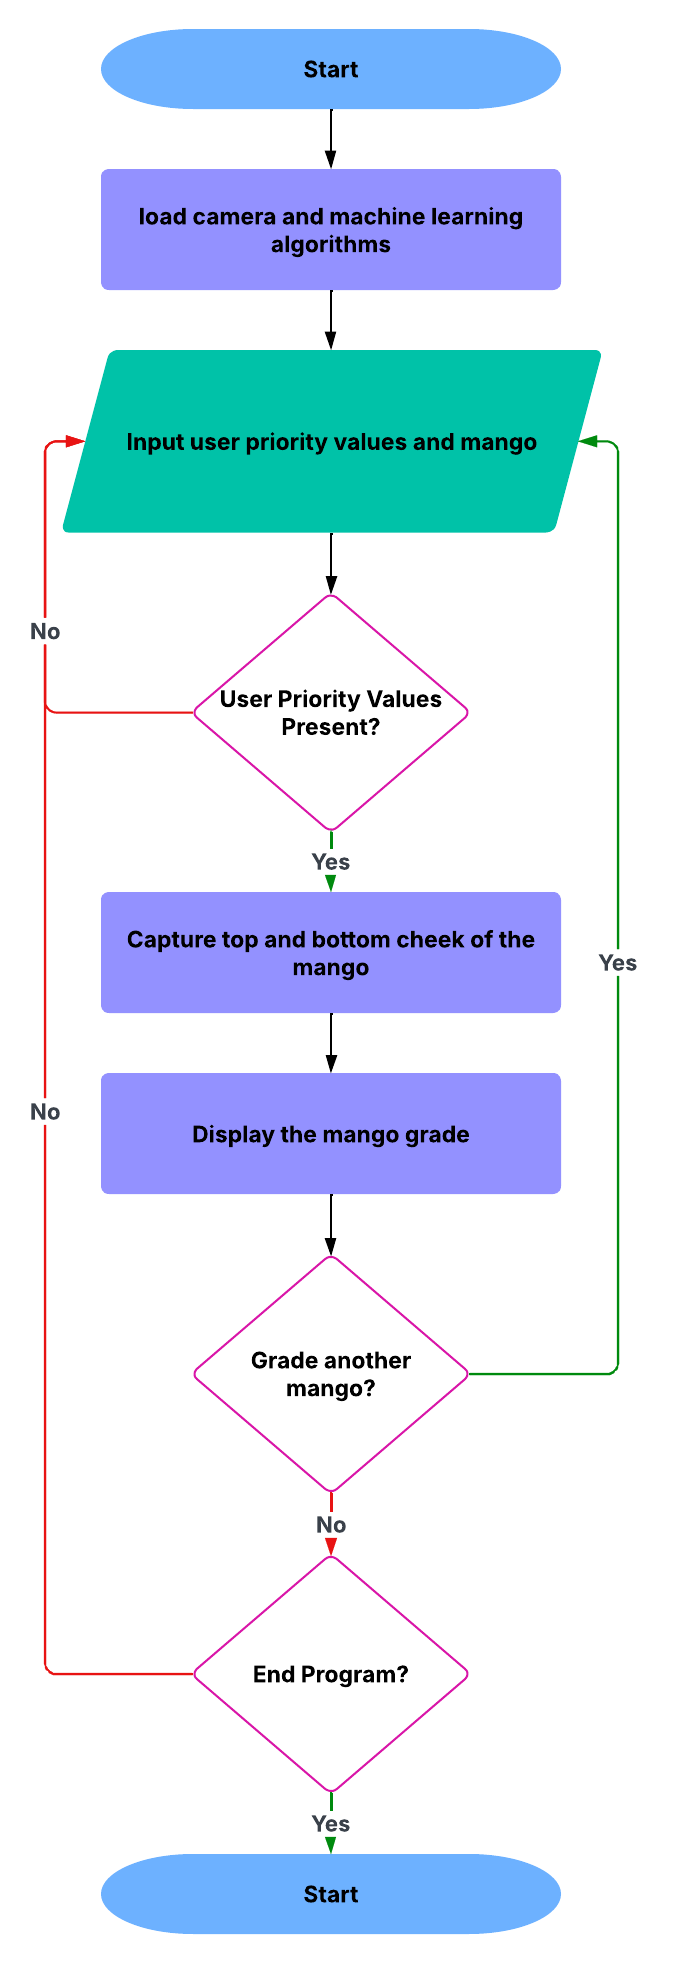
\includegraphics[width=0.40\textwidth]{mainFlowchart}
	\caption{Prototype Main Flowchart}
	\label{fig:pro2typeDiagram_fig}
\end{figure}

\subsection{Prototype 3D Model}
\begin{figure}[!htbp]
	\centering
	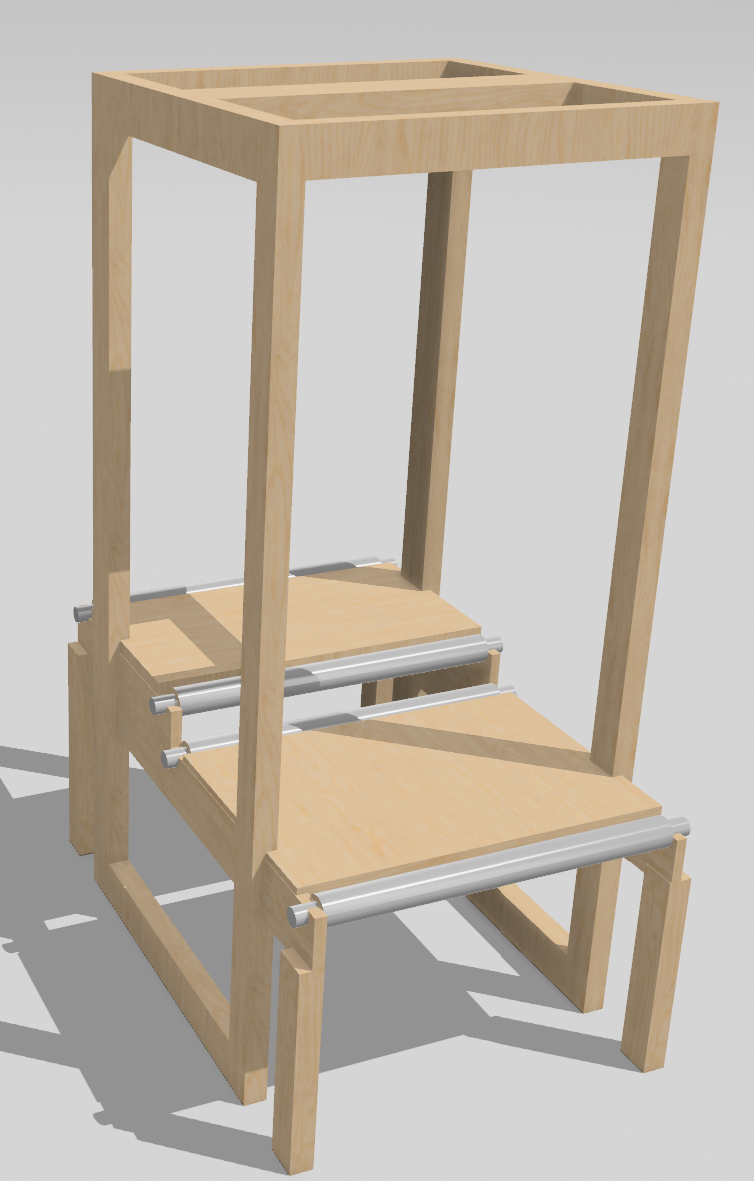
\includegraphics[width=0.60\textwidth]{3D_Drawing}
	\caption{Initial 3D Model of the Prototype}
	\label{fig:3dModel_fig}
\end{figure}


\subsection{Hardware Specifications}

\subsubsection{Raspberry Pi}
\begin{figure}[!htbp]
	\centering
	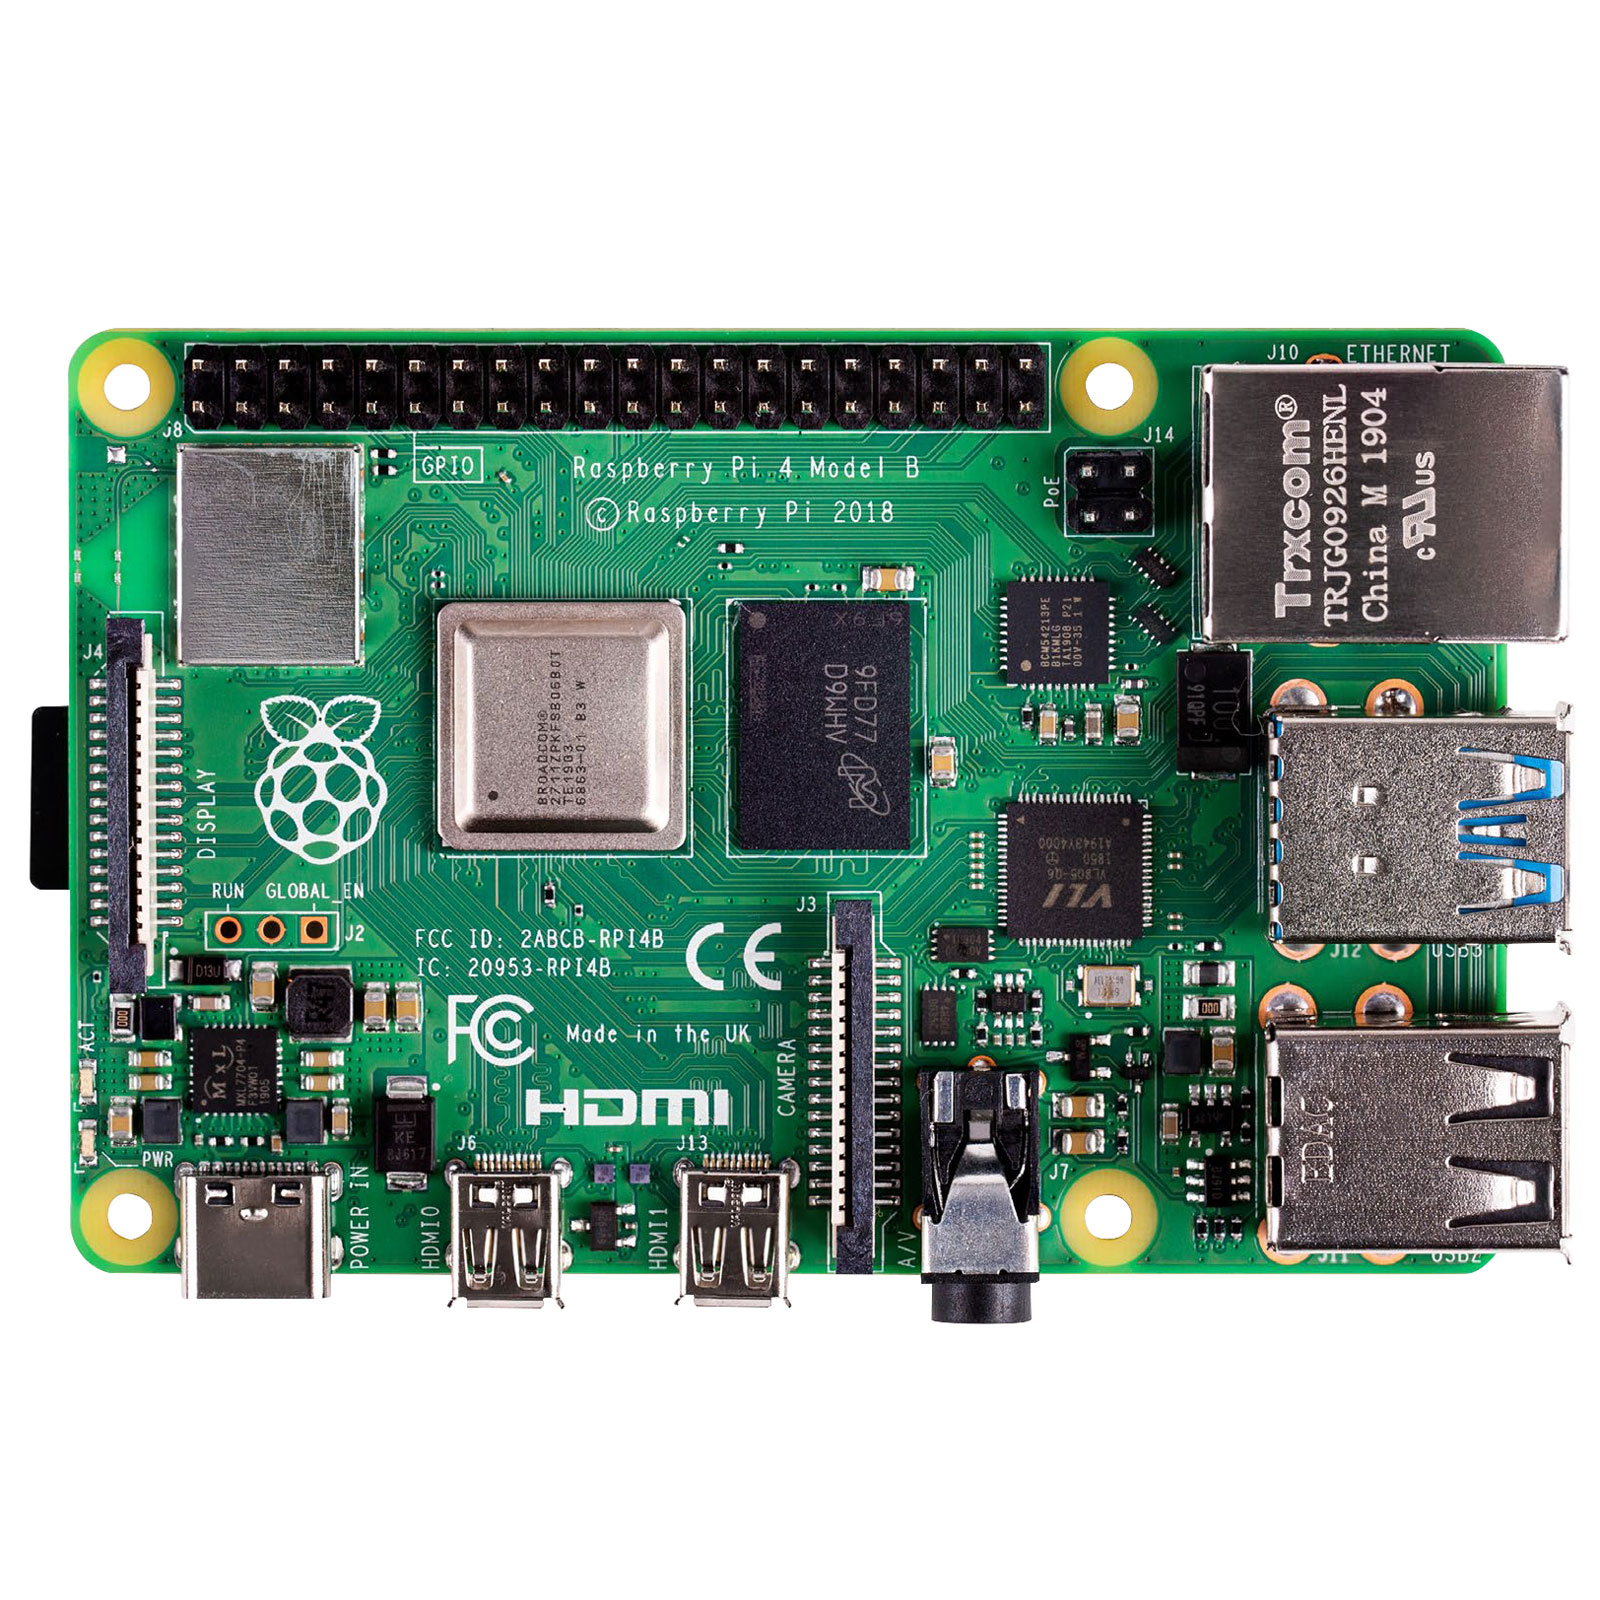
\includegraphics[width=0.5\textwidth]{rpi4b}
	\caption{Raspberry Pi 4 Model B}
	\label{fig:rpi4b_fig}
\end{figure}
The Raspberry Pi 4 Model B is a compact, low-cost computer that serves as the system's main processing unit. 
It was chosen for its balance of performance and affordability, making it suitable for image processing tasks.
Furthermore, it was selected for its compatibility with various peripherals through the GPIO pins and USB-A ports together
with its ease of integration into the prototype.
\\
\\
\textbf{Specifications:}
\begin{itemize}
    \item SoC: Broadcom BCM2711
    \item CPU: Quad-core ARM Cortex-A72 (64-bit)
    \item Clock Speed: 1.5 GHz (base, overclockable)
    \item RAM: 8GB LPDDR4-3200 SDRAM
    \item Wireless: Dual-band 2.4 GHz / 5 GHz Wi-Fi (802.11ac)
    \item Bluetooth: Bluetooth 5.0 (BLE support)
    \item Ethernet: Gigabit Ethernet (full throughput)
    \item USB: 2 x USB 3.0 ports and 2 x USB 2.0 ports
    \item Video Output: 2 x micro-HDMI ports (supports 4K @ 60Hz, dual 4K display capability)
    \item Audio: 3.5mm audio/video composite jack
    \item Storage: MicroSD card slot (supports booting via SD card or USB)
    \item GPIO: 40-pin GPIO header (backward-compatible with older models)
    \item Camera/Display: CSI (camera) and DSI (display) ports
    \item Power Input: USB-C (5V/3A recommended)
    \item Power Consumption: ~3W idle, up to 7.5W under load
\end{itemize}

\subsubsection{Raspberry Pi Camera}
\begin{figure}[!htbp]
	\centering
	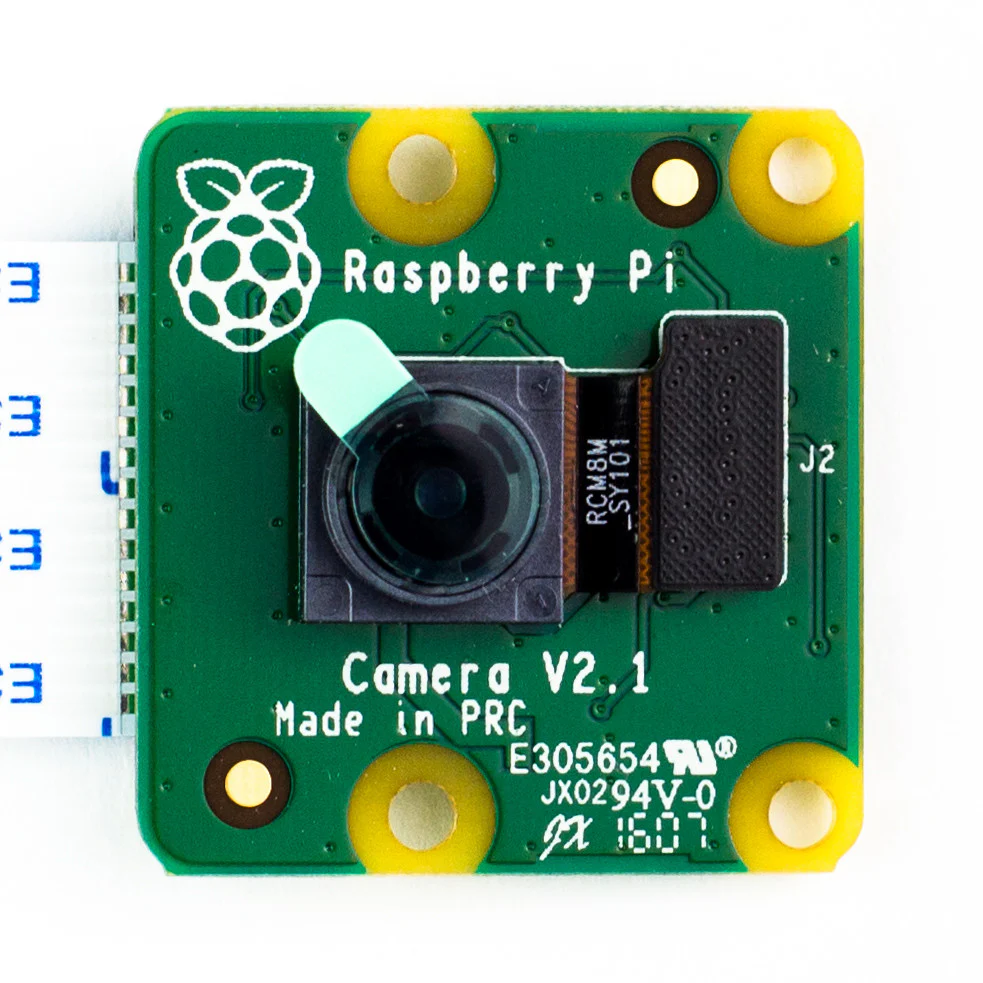
\includegraphics[width=0.5\textwidth]{rpi_cam}
	\caption{Raspberry Pi Camera Module Version 2}
	\label{fig:rpi_cam_fig}
\end{figure}
The Raspberry Pi Camera Module Version 2 is a high-quality camera module designed for the Raspberry Pi platform.
Likewise, it is capable of capturing still images at 8 megapixels, and supports video recording at 1080p @ 30fps, 
720p @ 60fps, and 480p @ 90fps. 
Moreover, it has a fixed-focus lens with a diagonal field of view of 62.2 degrees, and an optical format of 1/4 inch. 
Furthermore, it supports various Python libraries such as Picamera and OpenCV for image capture and processing.
As such, it was selected for its compact size, ease of integration, and ability to capture high-resolution images. 
\\
\\
\textbf{Specifications:}
\begin{itemize}
    \item Sensor: Sony IMX219PQ 8-megapixel CMOS sensor.
    \item Still Images Resolution: 8 MP (3280 x 2464 pixels).
    \item Video Resolution: Supports up to 1080p @ 30fps, 720p @ 60fps, and 480p @ 90fps.
    \item Focus: Fixed-focus lens (manual focus adjustment not supported without physical modification).
    \item Lens Size: 1/4-inch optical format.
    \item Field of View (FoV): Diagonal 62.2 degrees.
    \item Interface: Connected via 15-pin ribbon cable to the Raspberry Pi's CSI (Camera Serial Interface) port.
    \item APIs/Libraries: Supports Python libraries such as Picamera and OpenCV for image capture and processing.
    \item Dimensions: 25 mm x 24 mm x 9 mm.
\end{itemize}

\subsubsection{DC Motor}
\begin{figure}[!htbp]
	\centering
	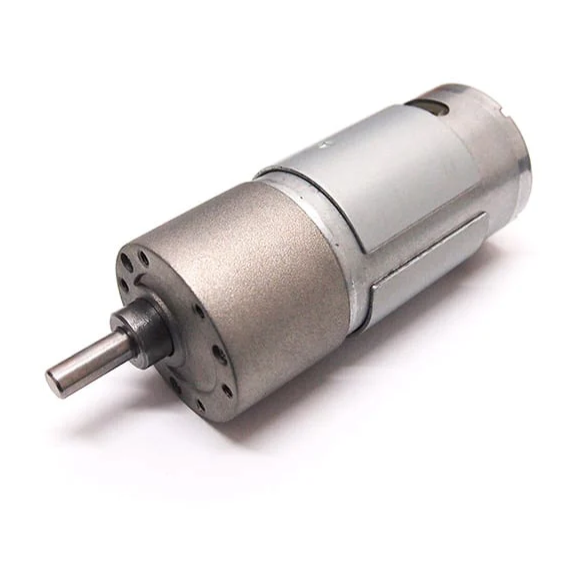
\includegraphics[width=0.5\textwidth]{dc_motor}
	\caption{12 Volt DC Gear Motor}
	\label{fig:dc_motor_fig}
\end{figure}
The 12 Volt DC Gear Motor is a compact, high-torque, and low-noise motor suitable for a 
wide range of applications, including robotics, automation, and industrial control systems. 
It features a spur gear design, which provides a high reduction ratio for increased torque output. 
The motor is designed for continuous operation and has a low power consumption under standard load 
conditions. Likewise, it is also capable of withstanding high temperatures and has a high reliability.
This motor was selected for its high torque output, low power consumption, and compact size, 
making it ideal for the conveyor system.
\\
\\
\textbf{Specifications:}
\begin{itemize}
    \item Gearbox Type: Spur gear design
    \item Operating Voltage: 12V (operational range: 6-12V)
    \item No-load Current Consumption: 0.8A
    \item Rated Current Draw: 3A (under standard load)
    \item No-load Speed: 282 RPM (maximum)
    \item Operating Speed: 248 RPM (under rated load)
    \item Torque Output: 18 kg-cm (rated)
    \item Stall Torque: 60 kg-cm (maximum)
    \item Power Rating: 50W (maximum)
    \item Unit Weight: 350 grams
\end{itemize}


\subsubsection{MicroSD Card}
\begin{figure}[!htbp]
	\centering
	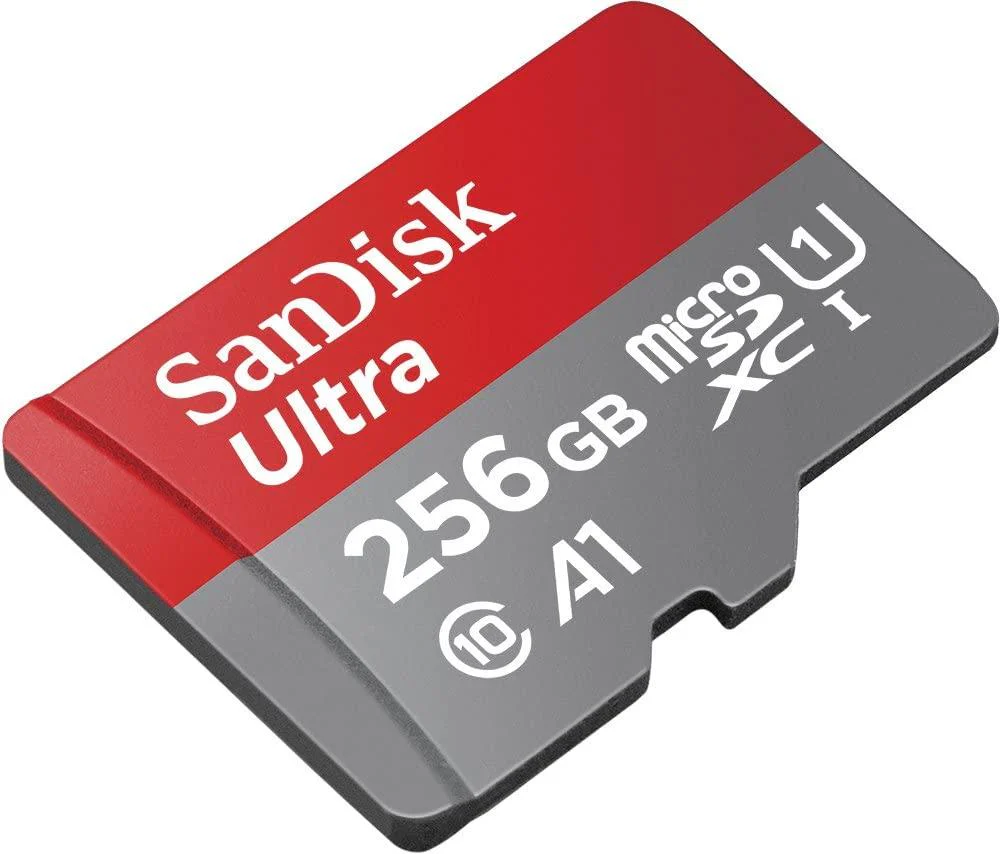
\includegraphics[width=0.5\textwidth]{sdCard}
	\caption{SanDisk Ultra MicroSD Card}
	\label{fig:sdCard_fig}
\end{figure}
The SanDisk Ultra MicroSD Card is a compact, high-capacity, and secure digital memory card 
that is suitable for a wide range of applications, including digital cameras, smartphones, and tablets.
It features a high-speed data transfer rate, making it ideal for storing large files such as images and videos.
This card was selected for its high capacity, secure data protection, and ease of use,
making it ideal for the storage system for the prototype. 
\\
\\
\textbf{Specifications:}
\begin{itemize}
    \item Capacity: 256GB
    \item Type: MicroSDXC (Secure Digital eXtended Capacity)
    \item Form Factor: MicroSD (11mm x 15mm x 1mm)
    \item File System: Pre-formatted exFAT
\end{itemize}

\subsubsection{LED Lights}
\begin{figure}[!htbp]
	\centering
	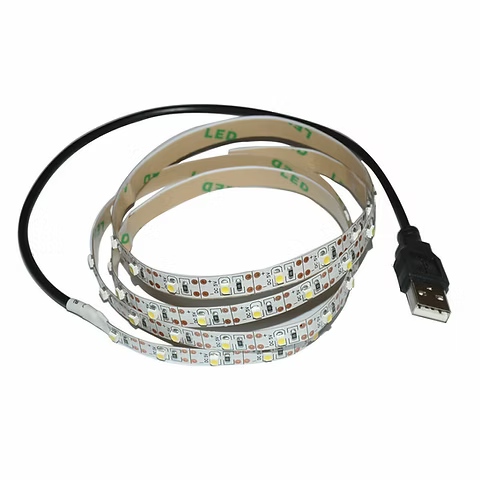
\includegraphics[width=0.5\textwidth]{led}
	\caption{LED Light Strip}
	\label{fig:led_fig}
\end{figure}
For the \gls{LED}, they were used to provide consistent lighting for image capture, ensuring accurate color representation and feature extraction.
The LED lights were selected for their energy efficiency, long lifespan, and ability to produce a uniform light output.
\\
\\
\textbf{Specifications:}
\begin{itemize}
    \item Power Input: 5V DC (USB-powered, compatible with laptops, power banks, or USB adapters).
    \item Waterproof Design: Suitable for indoor/outdoor use.
    \item LED Type: SMD 2835 (surface-mount diodes for high brightness and efficiency).
    \item Color Type: White (cool white)
    \item Length: 1m 
    \item Beam Angle: 120°
    \item Operating Temperature: -25°C to 60°C.
    \item Storage Temperature: -40°C to 80°C.
\end{itemize}


\subsubsection{Power Supply}
\begin{figure}[!htbp]
	\centering
	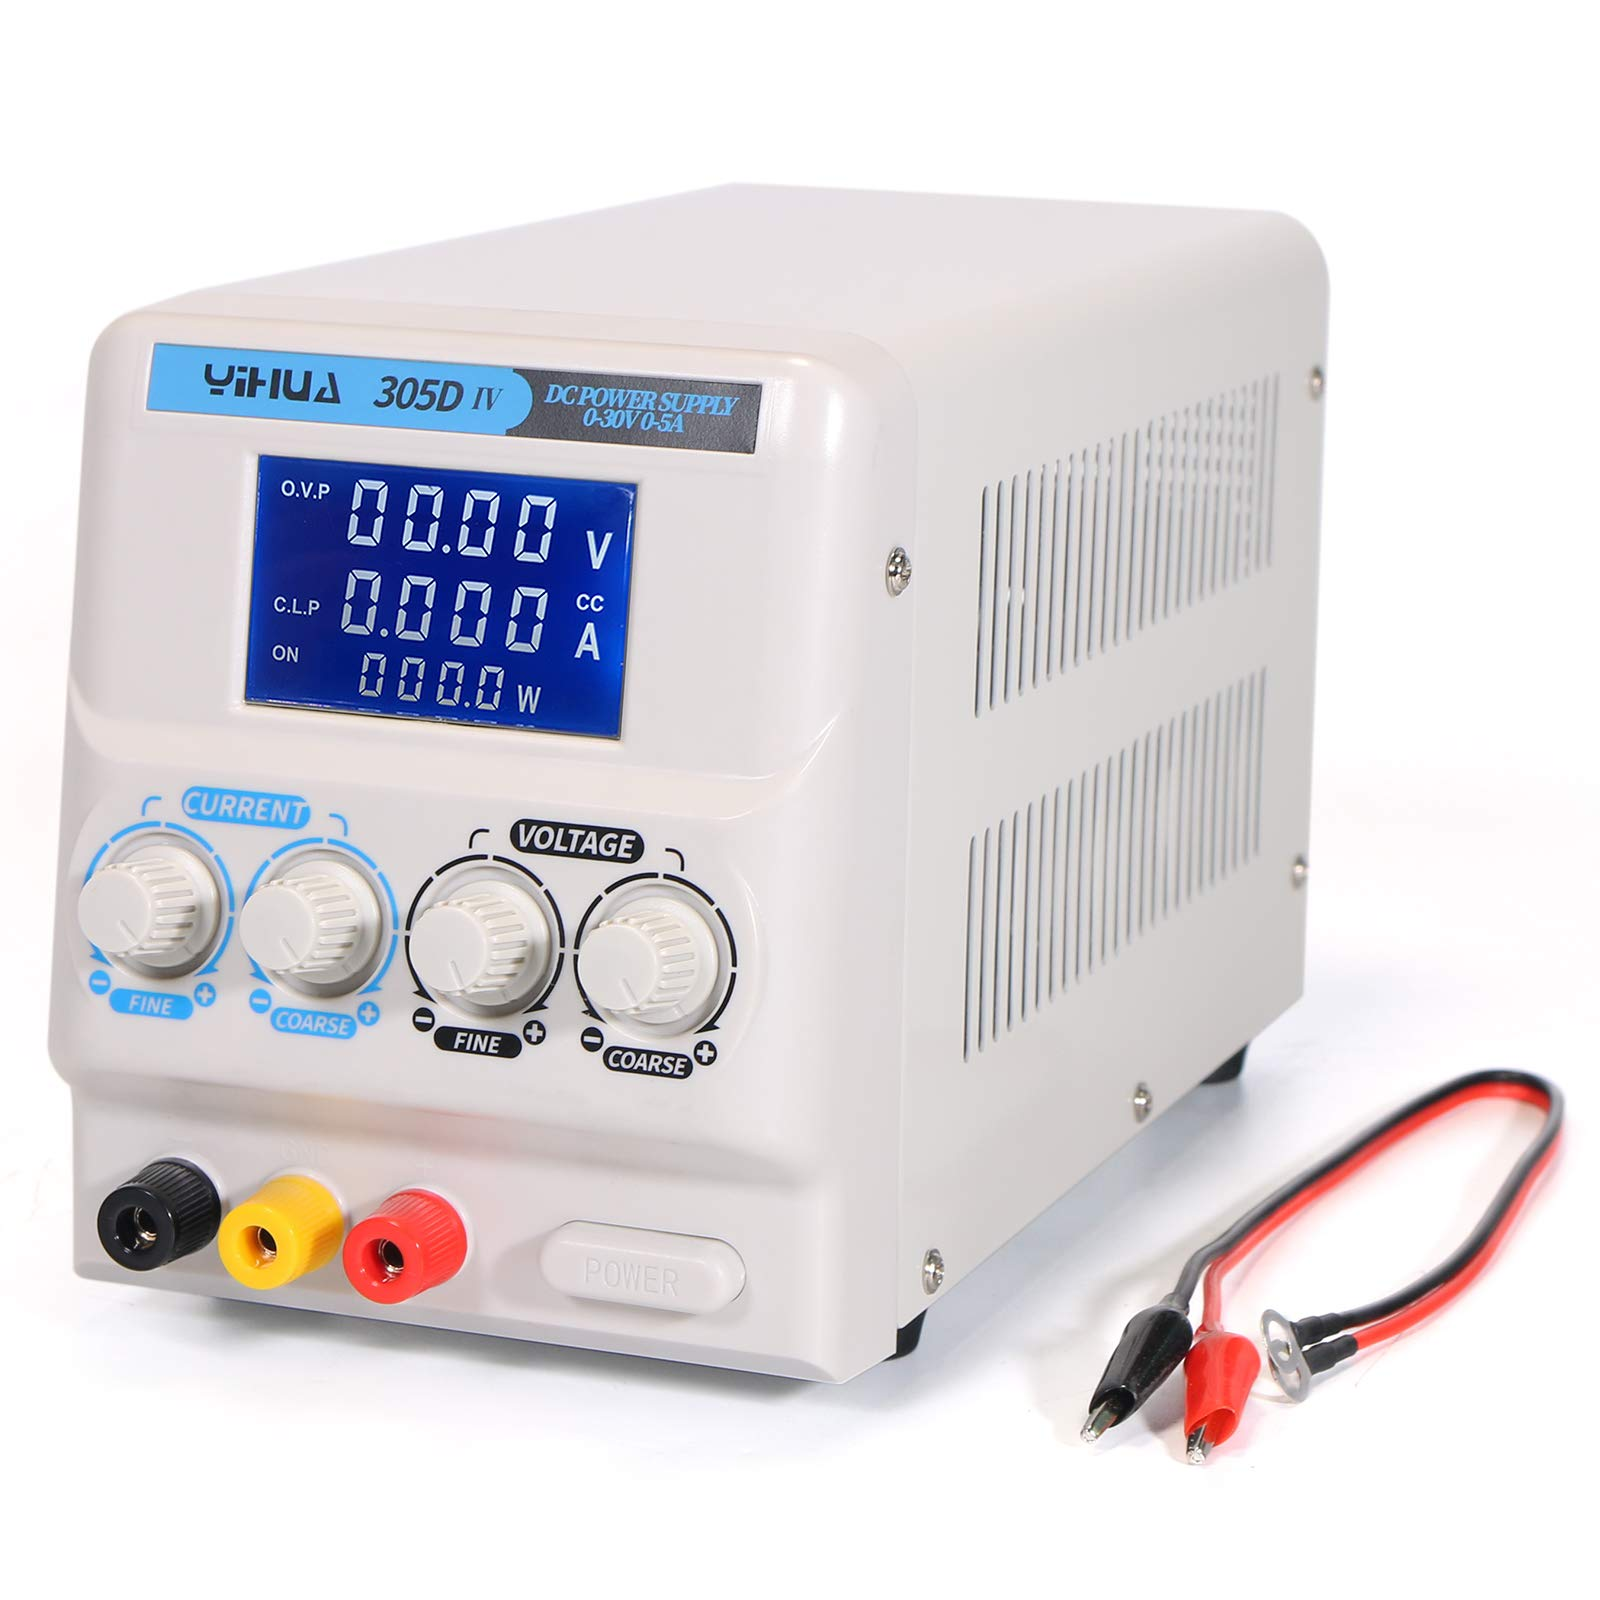
\includegraphics[width=0.5\textwidth]{Power_Supply}
	\caption{Bench Power Supply}
	\label{fig:Power_Supply_fig}
\end{figure}
The bench power supply is a versatile and adjustable power source used to 
provide stable voltage and current for various electronic projects.
It is designed for testing applications, allowing users to set specific voltage and current levels.
This power supply was selected for its versatility, 
ease of use, and ability to provide accurate voltage and current control for the prototype.
\\
\\
\textbf{Specifications:}
\begin{itemize}
    \item Type: SMPS (Switch-Mode Power Supply)
    \item Input: 110V AC, 50/60Hz (U.S. Standard)
    \item Output Range: 0-30V DC / 0-5A DC
    \item Voltage Precision: ±0.010V (10 mV) resolution
    \item Current Precision: ±0.001A (1 mA) resolution
    \item Power Precision: ±0.1W resolution
    \item Weight: 5 lbs (2.27 kg)
    \item Dimensions: 11.1" x 4.92" x 6.14" (28.2 cm x 12.5 cm x 15.6 cm)
    \item Maximum Power: 195W
    \item Power Source: AC input only
\end{itemize}

\subsubsection{4 Channel Relay Module}
\begin{figure}[!htbp]
	\centering
	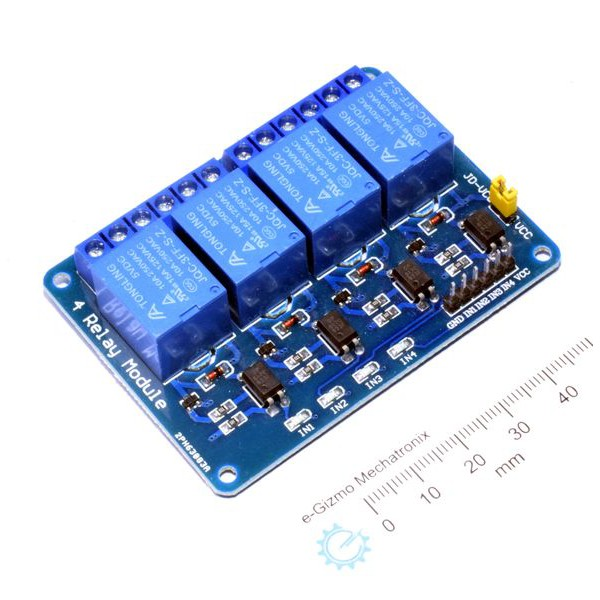
\includegraphics[width=0.5\textwidth]{relay_module}
	\caption{4 Channel Relay Module}
	\label{fig:relay_module_fig}
\end{figure}
The 4 Channel Relay Module is a compact and versatile relay 
board that allows for the control of multiple devices using a single microcontroller.
This module was selected for its compact size, ease of use, and ability to control multiple devices simultaneously.
It is designed to be used with microcontrollers such as Arduino and Raspberry Pi,
allowing for easy integration into the prototype.
\\
\\
\textbf{Specifications:}
\begin{itemize}
    \item Operating Voltage: 5V DC (compatible with Arduino, Raspberry Pi, and other microcontrollers).
    \item Number of Relays: 4 independent channels.
    \item Relay Type: Electromechanical (mechanical switching).
    \item Max AC Load: 10A @ 250V AC (resistive).
    \item Max DC Load: 10A @ 30V DC (resistive).
    \item Contact Type: SPDT (Single Pole Double Throw) - NO (Normally Open), NC (Normally Closed), COM (Common).
    \item Dimensions: ~50mm x 70mm x 20mm 
    \item Weight: ~50-80 grams.
    \item Status LEDs: Individual LEDs for each relay (indicates ON/OFF state).
    \item Input Pins: 4 digital control pins (one per relay).
    \item Output Terminals: Screw terminals for connecting loads (NO/NC/COM).
\end{itemize}

\section{Software Considerations}
The software stack includes Python for programming PyTorch for machine learning and OpenCV for image processing. These tools are selected for their robustness, ease of use, and extensive community support, ensuring efficient system development.

\subsection{PyTorch}

\subsection{OpenCV}

\subsection{Tkinter}

\subsection{CustomTkinter}

\section{Security and Reliability Considerations}
Potential vulnerabilities, such as data corruption during image capture, are addressed through redundancy and error-checking mechanisms. Reliability is ensured by implementing fault-tolerant designs and rigorous testing protocols.

\section{Scalability and Efficiency Considerations}
The system is designed to handle large volumes of mangoes by optimizing the machine learning model and using parallel processing techniques. Efficiency is improved through techniques like model quantization and hardware acceleration.

\section{User Interface}
A \gls{UI} is designed to display grading results, system status. Wireframes illustrate the layout, ensuring usability and accessibility for operators. 
Likewise, a \gls{GUI} is also used to allow users to customize the system's grading priorities.

\section{Constraints and Limitations}
Challenges include variations in mango appearance due to lighting and environmental factors. Trade-offs are made between model complexity and real-time performance to balance accuracy and speed.

\section{Technical Standards}
The system adheres to industry standards for image processing and machine learning, ensuring compatibility and interoperability with other systems.

\section{Prototyping and Simulation}
Prototypes are developed using tools like MATLAB and Simulink to simulate the system’s performance. These simulations help identify design flaws and optimize the system before deployment.,

\section{Design Validation}
The design is validated through testing, including unit testing of individual modules and integration testing of the entire system. Peer reviews and iterative improvements ensure the system meets the desired performance metrics.

\section{Summary}
This chapter outlined the key design considerations, including system architecture, hardware and software choices, and validation methods. These decisions are critical for developing a reliable and efficient mango sorting and grading system.


	%\stopcontents[chapters]
	\cleardoublepage
	
	%%%%%%%%%%%%%%%%%%%%%%%%%%%%%%%%%%%%%%%%%%%%%%%%
	\chapter{Methodology} 
	\label{ch:method} 
	%\startcontents[chapters]
	%\begin{SingleSpace}	
	%	\Mprintcontents 
	%\end{SingleSpace}
	
% \begin{center}
	% 	{\scriptsize
		% 		\begin{tabularx}{\textwidth}{p{0.2\textwidth}|p{0.6\textwidth}|p{0.1\textwidth}}
			% 			\caption{Summary of methods for reaching the objectives} \label{tab:methods_per_objective} \\
			% 			\hline 
			% 			\hline 
			% 			\textbf{Objectives} & 
			% 			\textbf{Methods} &
			% 			\textbf{Locations}\\ 
			% 			\hline 
			% 			\endfirsthead
			% 			\multicolumn{3}{c}%
			% 			{\textit{Continued from previous page}} \\
			% 			\hline
			% 			\hline 
			% 			\textbf{Objectives} & 
			% 			\textbf{Methods} &
			% 			\textbf{Locations}\\ 
			% 			\hline 
			% 			\endhead
			% 			\hline 
			% 			\multicolumn{3}{r}{\textit{Continued on next page}} \\ 
			% 			\endfoot
			% 			\hline 
			% 			\endlastfoot
			% 			\hline
			% 			
			% 			
			% 			\Paste{GO} & \blindlist{enumerate} & Sec.~\ref{sec:implement} on p.~\pageref{sec:implement}\\ \hline
			% 			
			% 			
			% 			\Paste{SO1} & \blindlist{enumerate} & Sec.~\ref{sec:implement} on p.~\pageref{sec:implement} \\ \hline
			% 			
			% 			
			% 			\Paste{SO2} & \blindlist{enumerate} & Sec.~\ref{sec:implement} on p.~\pageref{sec:implement}\\ \hline
			% 			
			% 			
			% 			\Paste{SO3} & \blindlist{enumerate} & Sec.~\ref{sec:implement} on p.~\pageref{sec:implement}\\ \hline
			% 			
			% 			
			% 			\Paste{SO4} & \blindlist{enumerate} & Sec.~\ref{sec:implement} on p.~\pageref{sec:implement} \\ \hline
			% 			
			% 			
			% 			\Paste{SO5} & \blindlist{enumerate} & Sec.~\ref{sec:implement} on p.~\pageref{sec:implement} \\ \hline
			% 			
			% 		\end{tabularx}
		% 	}
	% \end{center}

\section{Introduction}
The methodology for this research outlines the development of the Carabao Mango sorter using machine learning and computer vision. The sorting system uses a conveyor belt system which delivers the mangoes into the image acquisition system. This system captures the image of the mangoes which will then be going through the various stages of image processing and classification into grades which will depend on the priority of the user. This methodology ensures that the grading of the mangoes will be accurate while being non-destructive.

\section{Research Approach}
This study applies the experimental approach for research in order to develop and properly test the proposed system. The experimental approach of the methodology will allow the researchers to fine-tune the parameters and other factors in the classification of mangoes in order to get optimal results with high accuracy scores while maintaining the quality of the mangoes. This approach will also allow for real-time data processing and classification which will improve the previous static grading systems.

\section{Experimental Setup}
The prototype consists of hardware and software components for automated mango sorting and grading purposes. The hardware includes the conveyor belt system used to transfer mangoes from scanning to sorting smoothly. A camera and lighting system are able to collect high-resolution images for analysis. The DC motors and stepper motors are responsible for driving the conveyor belt and sorting actuators. The entire system is controlled by a microcontroller (Raspberry Pi 4b), coordinating actions of all components. Sorting actuators then direct mangoes into selected bins based on their classification to make sorting efficient. For the programming language used for the prototype and training and testing the CNN model, Python was used for training and testing the CNN model and it was also used in the microcontroller to run the application containing the UI and CNN model. PyTorch was the main library used in using the EfficientNet model that is used in classifying the ripeness and bruises of the mango. Likewise, tkinter is the used library when designing the UI in Python.

In addition to their hardware, the rest of the software components are of utmost importance to mango classification. Image processing algorithms in OpenCV and CNN models extract features such as color, size, and bruises that are known to determine quality parameters of mangoes. Mangoes are classified based on ripeness and defects by using machine learning algorithms, which further enhances accuracy using deep learning techniques. A user interface (UI) is designed for users to control and observe the system in real time. Finally, the interface programming of the microcontroller provides the necessary synchronization between sensors, actuators, and motors throughout the sorting operation scenario.

\section{Data Collection Methods}
The system acquires high-resolution images of mangoes under pre-specified lighting conditions through systematic acquisition. Apart from that, this corpus of data is based on the real-time images acquired from the camera system, where classification operations are carried out based on real-time data. Pre-processing image operations such as flipping, rotating, resizing, normalization, and Gaussian blur are also carried out in order to enhance image clarity and feature detection. Then, the feature extraction process is carried out, where the intensity of color, shape, and texture are analyzed for the detection of characteristic features in terms of the mango. All these aspects lead to the creation of a reliable dataset for the machine learning algorithm that will allow the system to classify and grade mangoes more accurately.

\section{Testing and Evaluation Methods}
In a bid to ensure the mango sorting and grading system is accurate and reliable, there is intensive testing conducted at different levels. Unit testing is initially conducted on each component separately, for instance, the conveyor belt, sensors, and cameras, to ensure that each of the components works as expected when operating separately. After component testing on an individual basis, integration testing is conducted to ensure communication between hardware and software is correct to ensure the image processing system, motors, and sorting actuators work in concert as required. System testing is conducted to conduct overall system performance testing in real-world conditions to ensure mangoes are accurately and efficiently sorted and graded.

\begin{eqnarray}
	\text{Precision} = \frac{TP}{TP + FP}
	\label{eq:precision}
\end{eqnarray}

\begin{eqnarray}
	\text{Recall} = \frac{TP}{TP + FN}
	\label{eq:recall}
\end{eqnarray}


To test system performance, various measures of performance are used to evaluate. As seen on equation~\ref{eq:accuracy}, accuracy is used to measure the percentage of correctly classified mangoes to ensure the system maintains high precision levels. Precision as seen on equation~\ref{eq:precision} and recall as seen on equation~\ref{eq:recall} are used to measure consistency of classification to determine if the system classifies different ripeness levels and defects correctly. Furthermore, the F1 score formula as seen on equation~\ref{eq:f1_score} is used to evaluate the performance of the model's classification. 

\begin{eqnarray}
	F_1 = 2\times \frac{\text{Precision} \times \text{Recall}}{\text{Precision} + \text{Recall}}
	\label{eq:f1_score}
\end{eqnarray}

\begin{eqnarray}
	\text{Accuracy} = \frac{TP + TN}{TP + TN + FP + FN}
	\label{eq:accuracy}
\end{eqnarray}

A confusion matrix is used to measure correct and incorrect classification to ensure the machine learning model is optimized and that minimum errors are achieved. Throughput analysis is also used to determine the rate and efficiency of sorting to ensure that the system maintains high capacity without bottlenecks to sort mangoes. Using these methods of testing, the system is constantly optimized to ensure high-quality and reliable mango classification.

\section{Ethical Considerations}
Ethical considerations ensure that the system is operated safely and responsibly. Data privacy is ensured by securely storing and anonymizing extracted images and classification data so that unauthorized access becomes impossible. The system is also eco-friendly through non-destructive testing, saving mangoes while also ensuring that they are of good quality. Safety in operations is also ensured by protecting moving parts to prevent mechanical harm and incorporating fail-safes to securely stop operation in case of malfunction. Addressing these concerns, the system is not only accurate and efficient but also secure, eco-friendly, and safe for operators, thus a sustainable solution to automated mango sorting and grading.

\section{Summary}
This chapter explained how to create an automatic Carabao mango sorter and grader using machine learning and computer vision. The system integrates hardware and software resources, including a conveyor belt, cameras, sensors, and actuators, to offer accurate, real-time sorting by ripeness, size, and bruises. Various testing and evaluation processes ensure its performance to offer reliability. Ethical issues are data privacy, environmental sustainability, and operation safety. With enhanced efficiency, reduced human error, and enhanced quality, this system provides an affordable, scalable, and non-destructive solution to post-harvest mango classification in agricultural industries.

	%\stopcontents[chapters]
	\cleardoublepage
	
	%%%%%%%%%%%%%%%%%%%%%%%%%%%%%%%%%%%%%%%%%%%%%%%%
	\ifResultDiscuss 
	\chapter{Results and Discussions} 
	%	\label{ch:result_discuss} 
	%	\startcontents[chapters]
	%	\begin{SingleSpace}	
	%		\Mprintcontents 
	%	\end{SingleSpace}
		
Show in this chapter proofs why your proposed solution works.  However, presenting results ("It worked") without an appropriate explanation does not show thorough understanding.  Aside from the data and results that you have obtained, and their explanation, the discussion includes why components of your proposed solution work did or did not work in accordance to what you described in the evaluation process, and how the proposed solution performed and faired. Interpret the results and the reasons why they were obtained.  If your results are incorrect, apparent discrepancies from theory should be pointed out and explained. In essence, what do the results mean?  Citing existing publication can help you compare your results and your explanations. 

The next items below is not related to the description of this results and discussions chapter, but serves as an opener for the \LaTeX portion of this template.


In aggregate form, Table~\ref{tab:outcomes_per_objective} shows the outcomes and completions in applying the methodology of the \documentType per objective. \begin{center}
	{\scriptsize
		\begin{tabularx}{\textwidth}{p{0.2\textwidth}|p{0.6\textwidth}|p{0.1\textwidth}}
			\caption{Summary of methods for reaching the objectives} \label{tab:methods_per_objective} \\
			\hline 
			\hline 
			\textbf{Objectives} & 
			\textbf{Methods} & 
			\textbf{Locations} \\ 
			\hline 
			\endfirsthead
			\multicolumn{3}{c}%
			{\textit{Continued from previous page}} \\
			\hline
			\hline 
			\textbf{Objectives} & 
			\textbf{Methods} & 
			\textbf{Locations} \\ 
			\hline 
			\endhead
			\hline 
			\multicolumn{3}{r}{\textit{Continued on next page}} \\ 
			\endfoot
			\hline 
			\endlastfoot
			\hline
			
			\Paste{GO} & 
			\begin{enumerate}
				\item Build an image acquisition system with a conveyor belt, LED lights, and Raspberry Pi Camera
				\item Coded a Raspberry Pi application to grade and sort the Carabao mangoes
			\end{enumerate} 
			& Sec.~\ref{sec:implement} on p.~\pageref{sec:implement} \\ \hline
			
			\Paste{SO1} & \begin{enumerate}
				\item Build a physical prototype 
				\item Developed a Raspberry Pi application to grade and sort the Carabao mangoes
			\end{enumerate} & Sec.~\ref{sec:implement} on p.~\pageref{sec:implement} \\ \hline
			
			\Paste{SO2} & \begin{enumerate}
				\item Trained and tested using a pre-trained CNN model (EfficientNet with Adam optimizer) to classify ripeness and bruises
				\item Classified ripeness into green, yellow-green, and yellow
				\item Classified bruises into bruised and not bruised
			\end{enumerate} & Sec.~\ref{sec:implement} on p.~\pageref{sec:implement} \\ \hline
			
			\Paste{SO3} & \begin{enumerate}
				\item Coded a Raspberry Pi application to control the image acquisition system and conveyor belt
				\item Used a pre-trained CNN model (EfficientNet with Adam optimizer) to classify ripeness and bruises
			\end{enumerate} & Sec.~\ref{sec:implement} on p.~\pageref{sec:implement} \\ \hline
			
			\Paste{SO4} & \begin{enumerate}
				\item Formulated a linear equation based on the inputted user priority and the predicted mango classification
			\end{enumerate} & Sec.~\ref{sec:implement} on p.~\pageref{sec:implement} \\ \hline
			
			\Paste{SO5} & \begin{enumerate}
				\item Used a pre-trained CNN model (EfficientNet with Adam optimizer) to classify ripeness and bruises
				\item Applied computer vision techniques such as foreground mask and thresholding
			\end{enumerate} & Sec.~\ref{sec:implement} on p.~\pageref{sec:implement} \\ \hline
			
		\end{tabularx}
	}
\end{center}



\section{Summary}

Provide the gist of this chapter such that it reflects the contents and the message.
	%	\stopcontents[chapters]
	\cleardoublepage
	\fi
	
	%%%%%%%%%%%%%%%%%%%%%%%%%%%%%%%%%%%%%%%%%%%%%%%%
	\ifConc
	\chapter{Conclusions, Recommendations, and Future Directives} 
	\label{ch:conc} 
	%	\startcontents[chapters]
	%	\begin{SingleSpace}	
	%		\Mprintcontents 
	%	\end{SingleSpace}
		\section{Concluding Remarks}

In this \documentType, \ldots

Put here the main points that should be known and learned about the  work topic. Summarize or give the gist of the essential principles and inferences drawn from your results.

\section{Contributions}

The interrelated \index{contributions} contributions and supplements that have been developed by the author(s) in this \documentType \ are listed as follows.  Only those that are unique to the authors' work are included.

\begin{itemize}
  \item the ; 
	
	\item the ; 
  
  \item the ; 
	
\end{itemize}


\section{Recommendations}

\graytx{\Blindtext}

\section{Future Prospects}

There are several prospects that may be extended for further studies. \ldots So the suggested topics are listed in the following.

\begin{enumerate}
	\item  the \ldots.
	
	\item  the \ldots.
		
	\item  the \ldots.
\end{enumerate}

Note that for ECE undergraduate theses, as per the directions of the thesis adviser, Recommendations and Future Directives will be removed for the hardbound copy but will be retained for database storage.


	%	\stopcontents[chapters]
	\cleardoublepage
	\fi
	
	%%%%%%%%%%%%%%%%%%%%%%%%%%%%%%%%%%%%%%%%%%%%%%%
	\renewcommand{\UrlFont}{\normalfont}
	%\bibliographystyle{IEEEtr} % for IEEE referencing format
	\bibliographystyle{apalike} % for APA referencing format
	\begin{SingleSpace}
		{\small \bibliography{references}}

		
	\end{SingleSpace}
	\vfill
	\begin{flushright}
		Produced: \usdate\today, \currenttime \\
	\end{flushright}
	\cleardoublepage 
	
	%%%%%%%%%%%%%%%%%%%%%%%%%%%%%%%%%%%%%%%%%%%%%%%%
	\SingleSpacing
	\appendix
	\renewcommand{\thechapter}{\Alph{chapter}}
	\renewcommand{\thesection}{\thechapter\arabic{section}}
	\appto\appendix{\renewcommand\thechapter{\AlphAlph{\value{chapter}}}} % for increasing appendix chapters beyond Z, i.e. AA, AB, etc.
	
	%%%%%%%%%%%%%%%%%%%%%%%%%%%%%%%%%%%%%%%%%%%%%%%%
	\chapter{Student Research Ethics Clearance}
	
\includepdf[pages={1},%
	offset=3.5mm -10mm,%
	scale=0.75,%
	pagecommand={},]
	{./figure/STUDENT_RESEARCH_ETHICS_CLEARANCE.pdf}
	\cleardoublepage
	
	%%%%%%%%%%%%%%%%%%%%%%%%%%%%%%%%%%%%%%%%%%%%%%%%
	\chapter{Answers to Questions to this \documentType}
	%\startcontents[chapters]
	%\Mprintcontents 
	


\refstepcounter{section}\section*{\thesection\quad  How important is the problem to practice?}

A possible answer to this question is the summary of your Significance of the Study, and that portion of the Problem Statement where you describe the ideal scenario for your intended audience. 

\graytx{\blindtext}
	
	
	
	
\refstepcounter{section}\section*{\thesection\quad  How will you know if the solution/s that you will achieve would be better than existing ones?}	

\graytx{\blindtext}


\refstepcounter{subsection}\subsection*{\thesubsection\quad How will you measure the improvement/s?}	

\graytx{\blindtext}

	
\refstepcounter{subsubsection}\subsubsection*{\thesubsubsection\quad  What is/are your basis/bases for the improvement/s?}

\graytx{\blindtext}
	
		
\refstepcounter{subsubsection}\subsubsection*{\thesubsubsection\quad  Why did you choose that/those basis/bases?}

\graytx{\blindtext}

				
\refstepcounter{subsubsection}\subsubsection*{\thesubsubsection\quad  How significant are your measure/s of the improvement/s?}

\graytx{\blindtext}






	
\refstepcounter{section}\section*{\thesection\quad What is the difference of the solution/s from existing ones?}
	
\graytx{\blindtext}

\refstepcounter{subsection}\subsection*{\thesubsection\quad How is it different from previous and existing ones?}

\graytx{\blindtext}
	
	
	
	
	
	
\refstepcounter{section}\section*{\thesection\quad What are the assumptions made (that are behind for your proposed solution to work)?}
	
\graytx{\blindtext}
		
	
\refstepcounter{subsection}\subsection*{\thesubsection\quad Will your proposed solution/s be sensitive to these assumptions?}
	
\graytx{\blindtext}

  
\refstepcounter{subsection}\subsection*{\thesubsection\quad Can your proposed solution/s be applied to more general cases when some assumptions are eliminated? If so, how?}

\graytx{\blindtext}






\refstepcounter{section}\section*{\thesection\quad What is the necessity of your approach / proposed solution/s?}

\graytx{\blindtext}
	
	
\refstepcounter{subsection}\subsection*{\thesubsection\quad What will be the limits of applicability of your proposed~solution/s?}

\graytx{\blindtext}
				
						
\refstepcounter{subsection}\subsection*{\thesubsection\quad What will be the message of the proposed solution to technical people?  How about to non-technical managers and busines people?}
			
\graytx{\blindtext}





\refstepcounter{section}\section*{\thesection\quad How will you know if your proposed solution/s is/are correct?}

\graytx{\blindtext} 
			
			
\refstepcounter{subsection}\subsection*{\thesubsection\quad Will your results warrant the level of mathematics used (i.e., will the end justify the means)?}
	    
\graytx{\blindtext}
			





\refstepcounter{section}\section*{\thesection\quad Is/are there an/\_ alternative way/s to get to the same solution/s?}

\graytx{\blindtext}
	
	
\refstepcounter{subsection}\subsection*{\thesubsection\quad Can you come up with illustrating examples, or even better, counterexamples to your proposed solution/s?}

\graytx{\blindtext}
	
	
\refstepcounter{subsection}\subsection*{\thesubsection\quad Is there an approximation that can arrive at essentially the same proposed solution/s more easily?}
	
\graytx{\blindtext}
			
	
	
	
	
\refstepcounter{section}\section*{\thesection\quad If you were the examiner of your \documentType, how would you present the \documentType \ in another way?  Give your remarks, especially for your methodology and the results and discussions.}

% \MakeTextLowercase{\documentType} currently fails inside section{}
	
\graytx{\blindtext}
	
	
\refstepcounter{subsection}\subsection*{\thesubsection\quad What are the weaknesses of your \documentType, specifically  your methodology and the results and discussions?}

\graytx{\blindtext}

	%\stopcontents[chapters]
	\cleardoublepage
	
	%%%%%%%%%%%%%%%%%%%%%%%%%%%%%%%%%%%%%%%%%%%%%%%%
	\chapter{Revisions to the Proposal} 
	\label{ch:revisions_to_the_proposal}
	%\startcontents[chapters]
	%\Mprintcontents  
	%Make a table with the following columns for showing the summary of revisions to the proposal based on the comments of the panel of examiners. 
\begin{enumerate}
	\item  Examiner
	\item  Comment
	\item  Summary of how the comment was addressed
	\item  Locations in the document where the changes have been reflected
\end{enumerate}


\begin{center}
{\scriptsize
\begin{tabularx}{\textwidth}{p{0.1\textwidth}|p{0.2\textwidth}|p{0.5\textwidth}|p{0.1\textwidth}}
\caption{Summary of Revisions to the Proposal} \label{tab:rev_proposal} \\
\hline 
\hline 
\textbf{Examiner} & 
\textbf{Comment} & 
\textbf{Summary of how the comment was addressed} &
\textbf{Locations} \\ 
\hline 
\endfirsthead
\multicolumn{4}{c}%
{\textit{Continued from previous page}} \\
\hline
\hline 
\textbf{Examiner} & 
\textbf{Comment} & 
\textbf{Summary of how the comment was addressed} &
\textbf{Locations} \\  
\hline 
\endhead
\hline 
\multicolumn{4}{r}{\textit{Continued on next page}} \\ 
\endfoot
\hline 
\endlastfoot

\documentAdviserTitle\ \documentAdviser &
\graytx{\blindtext} &
\graytx{\blindtext \blinddescription} &
Sec.~\ref{sec:implement} on p.~\pageref{sec:implement}, Sec.~\ref{sec:evaluate} on p.~\pageref{sec:evaluate}, Fig.~\ref{fig:exampletc} on p.~\pageref{fig:exampletc}\\
\hline 

\examinerChairTitle\ \examinerChair & 
\graytx{\blindtext} &
\graytx{\blindtext \blinddescription} &
Sec.~\ref{sec:implement} on p.~\pageref{sec:implement}, Sec.~\ref{sec:evaluate} on p.~\pageref{sec:evaluate}, Fig.~\ref{fig:exampletc} on p.~\pageref{fig:exampletc}\\
\hline 

\examinerATitle\ \examinerA & 
\graytx{\blindtext} &
\graytx{\blindtext \blinditemize} &
Sec.~\ref{sec:implement} on p.~\pageref{sec:implement}, Sec.~\ref{sec:evaluate} on p.~\pageref{sec:evaluate}, Fig.~\ref{fig:exampletc} on p.~\pageref{fig:exampletc}\\
\hline 

\examinerBTitle\ \examinerB & 
\graytx{\blindtext} &
\graytx{\blindtext \blindenumerate} &
Sec.~\ref{sec:implement} on p.~\pageref{sec:implement}, Sec.~\ref{sec:evaluate} on p.~\pageref{sec:evaluate}, Fig.~\ref{fig:exampletc} on p.~\pageref{fig:exampletc}\\
\hline 

\examinerCTitle\ \examinerC & 
\graytx{\blindtext} &
\graytx{\blindtext \blindmathtrue} &
Sec.~\ref{sec:implement} on p.~\pageref{sec:implement}, Sec.~\ref{sec:evaluate} on p.~\pageref{sec:evaluate}, Fig.~\ref{fig:exampletc} on p.~\pageref{fig:exampletc}\\
\hline 

\end{tabularx}
}
\end{center}
	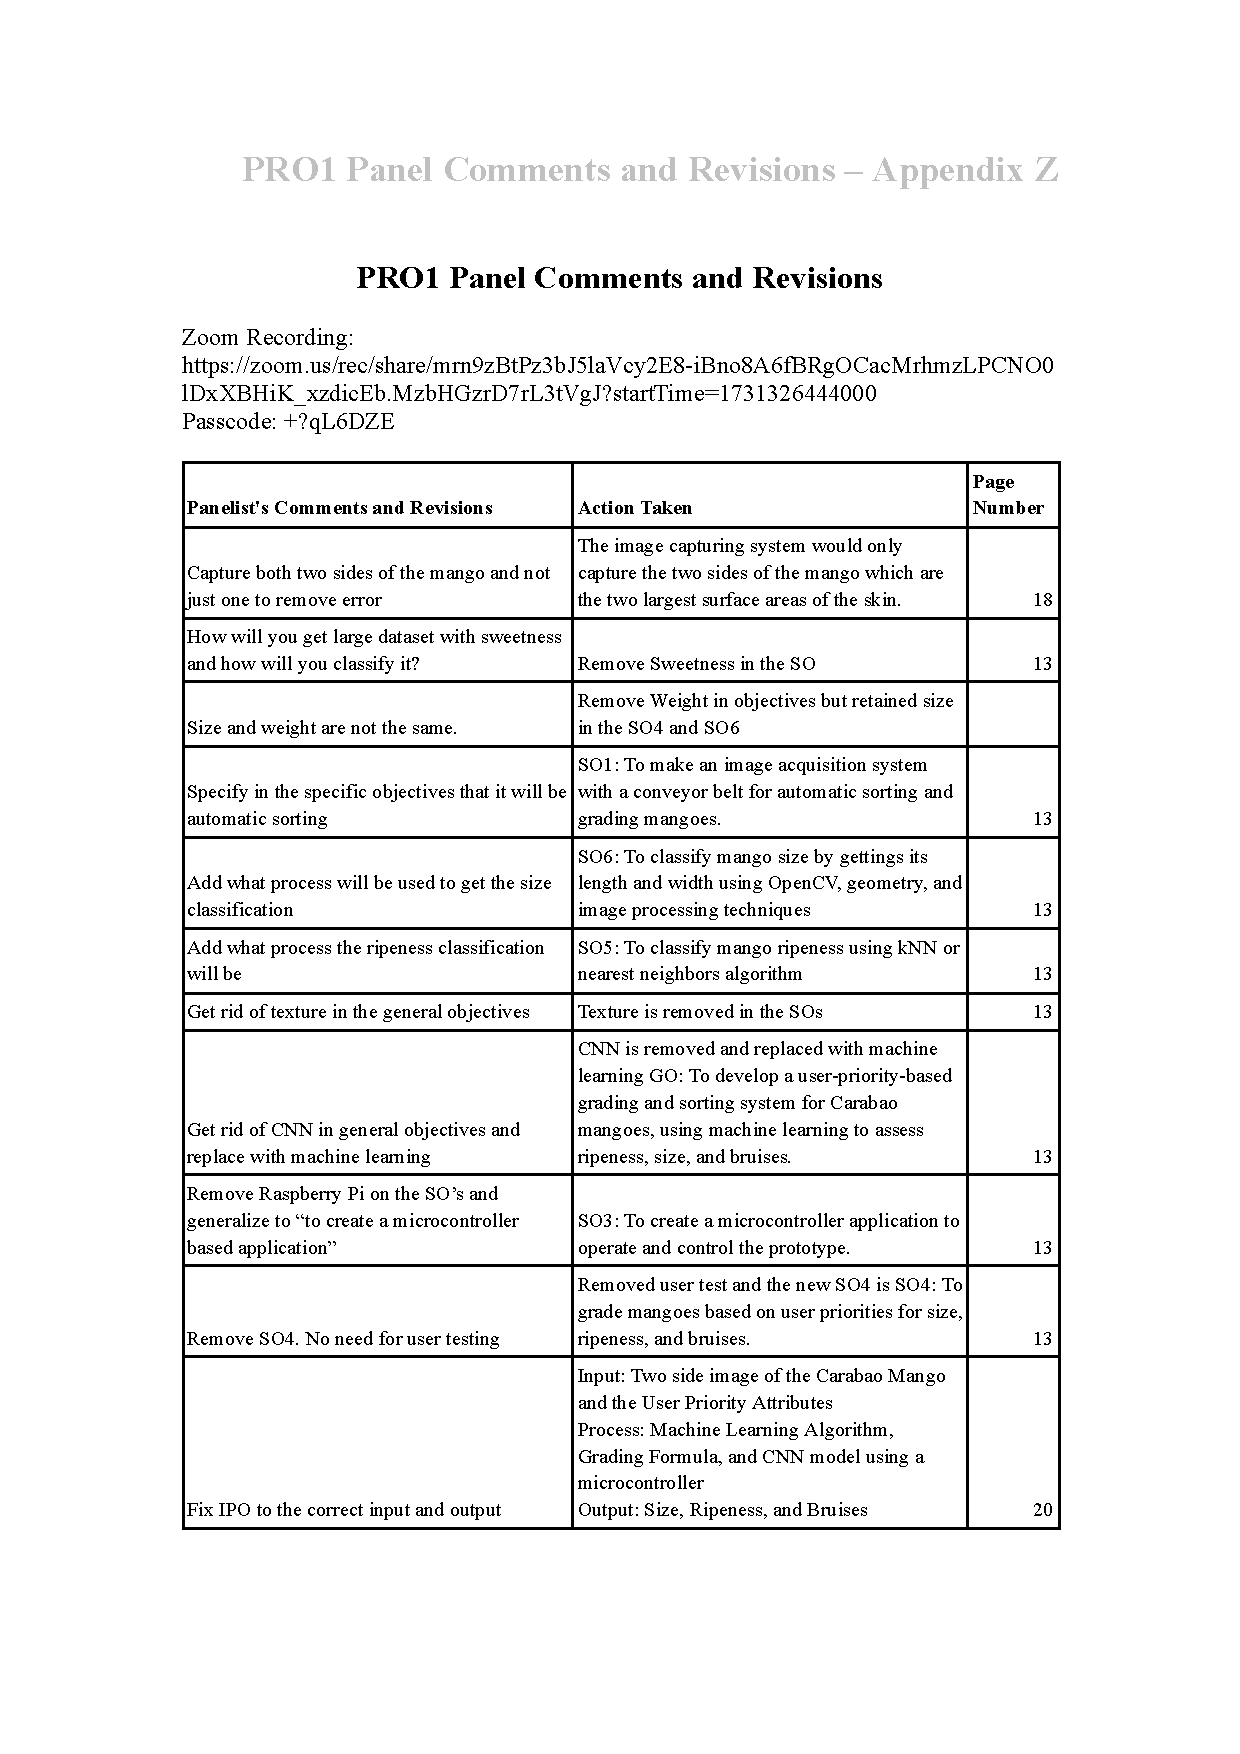
\includepdf[pages={1-5},
	offset=3.5mm -10mm,%
	scale=0.75,%
	pagecommand={},
	]{./figure/AppendixZ.pdf} % Includes all pages (1 to 5)
	%\stopcontents[chapters]
	\cleardoublepage
	
	%%%%%%%%%%%%%%%%%%%%%%%%%%%%%%%%%%%%%%%%%%%%%%%%
	\chapter{Revisions to the Final} 
	\label{ch:revisions_to_the_final}
	%\startcontents[chapters]
	%\Mprintcontents  
	Make a table with the following columns for showing the summary of revisions to the proposal based on the comments of the panel of examiners. 
\begin{enumerate}
	\item  Examiner
	\item  Comment
	\item  Summary of how the comment has been addressed
	\item  Locations in the document where the changes have been reflected
\end{enumerate}


\begin{center}
{\scriptsize
\begin{tabularx}{\textwidth}{p{0.1\textwidth}|p{0.2\textwidth}|p{0.5\textwidth}|p{0.1\textwidth}}
\caption{Summary of Revisions to the \documentType} \label{tab:rev_final} \\

\hline 
\hline 
\textbf{Examiner} & 
\textbf{Comment} & 
\textbf{Summary of how the comment has been addressed} &
\textbf{Locations} \\ 
\hline 
\endfirsthead
\multicolumn{4}{c}%
{\textit{Continued from previous page}} \\

\hline
\hline 
\textbf{Examiner} & 
\textbf{Comment} & 
\textbf{Summary of how the comment has been addressed} &
\textbf{Locations} \\  
\hline 
\endhead
\hline 
\multicolumn{4}{r}{\textit{Continued on next page}} \\ 

\endfoot
\hline 
\endlastfoot

\documentAdviserTitle\ \documentAdviser &
\graytx{\blindenumerate} &
\graytx{\blindenumerate \blinddescription} &
Sec.~\ref{sec:implement} on p.~\pageref{sec:implement}, Sec.~\ref{sec:evaluate} on p.~\pageref{sec:evaluate}, Fig.~\ref{fig:exampletc} on p.~\pageref{fig:exampletc}\\
\hline 

\examinerChairTitle\ \examinerChair & 
\graytx{\blindenumerate} &
\graytx{\blindenumerate \blinddescription} &
Sec.~\ref{sec:implement} on p.~\pageref{sec:implement}, Sec.~\ref{sec:evaluate} on p.~\pageref{sec:evaluate}, Fig.~\ref{fig:exampletc} on p.~\pageref{fig:exampletc}\\
\hline \\

\examinerATitle\ \examinerA & 
\graytx{\blindenumerate} &
\graytx{\blindenumerate \blinditemize} &
Sec.~\ref{sec:implement} on p.~\pageref{sec:implement}, Sec.~\ref{sec:evaluate} on p.~\pageref{sec:evaluate}, Fig.~\ref{fig:exampletc} on p.~\pageref{fig:exampletc}\\
\hline 

\examinerBTitle\ \examinerB & 
\graytx{\blindenumerate} &
\graytx{\blindenumerate} &
Sec.~\ref{sec:implement} on p.~\pageref{sec:implement}, Sec.~\ref{sec:evaluate} on p.~\pageref{sec:evaluate}, Fig.~\ref{fig:exampletc} on p.~\pageref{fig:exampletc}\\
\hline 

\examinerCTitle\ \examinerC & 
\graytx{\blindenumerate} &
\graytx{\blindenumerate \blindmathtrue} &
Sec.~\ref{sec:implement} on p.~\pageref{sec:implement}, Sec.~\ref{sec:evaluate} on p.~\pageref{sec:evaluate}, Fig.~\ref{fig:exampletc} on p.~\pageref{fig:exampletc}\\
\hline 

\end{tabularx}
}
\end{center}
	%\stopcontents[chapters]	
	\cleardoublepage
	
	%%%%%%%%%%%%%%%%%%%%%%%%%%%%%%%%%%%%%%%%%%%%%%%%
	%\chapter{Usage Examples} 
	%\label{ch:usage_examples}
	%\startcontents[chapters]
	%\Mprintcontents  
	%The user is expected to have a working knowledge of \LaTeX. A good introduction is in~\cite{Oetiker2014}.  Its latest version can be accessed at \url{http://www.ctan.org/tex-archive/info/lshort}.




\section{Equations}
\label{sec:eqn_not}

The following examples show how to typeset equations in \LaTeX.  This section also shows examples of the use of \verb| \gls{ } | commands in conjunction with the items that are in the \verb| notation.tex | file. \textbf{Please make sure that the entries in} \verb| notation.tex |\textbf{  are those that are referenced in the \LaTeX \ document files used by this \documentType.  Please comment out unused notations and be careful with the commas and brackets  in} \verb| notation.tex |.

In~\eqref{eq:conv}, the output signal \gls{not:output_sigt} is the result of the convolution of the input signal \gls{not:input_sigt} and the impulse response \gls{not:ir}.

\begin{eqnarray}   
     y\left( t \right) = h\left( t \right) * x\left( t \right)=\int_{-\infty}^{+\infty}h\left( t-\tau \right)x\left( \tau \right) \mathrm{d}\tau
	\label{eq:conv}
\end{eqnarray}

Other example equations are as follows.

\begin{eqnarray}
	\left[ \dfrac{ V_{1} }{ I_{1} } \right] = 
	\begin{bmatrix}
		A & B \\ 
		C & D 
	\end{bmatrix} 
	\left[ \dfrac{ V_{2} }{ I_{2} } \right]
	\label{eq:ABCD}
\end{eqnarray}

\begin{eqnarray}
\dfrac{1}{2} < \left\lfloor \mathrm{mod}\left(\left\lfloor \dfrac{y}{17} \right\rfloor 2^{-17 \lfloor x \rfloor - \mathrm{mod}(\lfloor y\rfloor, 17)},2\right)\right\rfloor,
\end{eqnarray}

\begin{eqnarray}
| \zeta(x)^3 \zeta(x + iy)^4 \zeta(x + 2iy) | = 
\exp\sum_{n,p} \frac{3 + 4 \cos( ny \log p) + \cos (2ny \log p)}{np^{nx}} \ge 1
\end{eqnarray}

\newpage
The verbatim \LaTeX \ code of Sec.~\ref{sec:eqn_not} is in List.~\ref{lst:eqn_gls}.

\begin{lstlisting}[
float=h,
caption=Sample \LaTeX \ code for equations and notations usage, 
label=lst:eqn_gls,
language=TeX,
frame=single]
The following examples show how to typeset equations in \LaTeX.  This section also shows examples of the use of \verb| \gls{ } | commands in conjunction with the items that are in the \verb| notation.tex | file. \textbf{Please make sure that the entries in} \verb| notation.tex |\textbf{  are those that are referenced in the \LaTeX \ document files used by this \documentType.  Please comment out unused notations and be careful with the commas and brackets  in} \verb| notation.tex |.

In~\eqref{eq:conv}, the output signal \gls{not:output_sigt} is the result of the convolution of the input signal \gls{not:input_sigt} and the impulse response \gls{not:ir}.

\begin{eqnarray}   
     y\left( t \right) = h\left( t \right) * x\left( t \right)=\int_{-\infty}^{+\infty}h\left( t-\tau \right)x\left( \tau \right) \mathrm{d}\tau
	\label{eq:conv}
\end{eqnarray}

Other example equations are as follows.

\begin{eqnarray}
	\left[ \dfrac{ V_{1} }{ I_{1} } \right] = 
	\begin{bmatrix}
		A & B \\ 
		C & D 
	\end{bmatrix} 
	\left[ \dfrac{ V_{2} }{ I_{2} } \right]
	\label{eq:ABCD}
\end{eqnarray}

\begin{eqnarray}
\dfrac{1}{2} < \left\lfloor \mathrm{mod}\left(\left\lfloor \dfrac{y}{17} \right\rfloor 2^{-17 \lfloor x \rfloor - \mathrm{mod}(\lfloor y\rfloor, 17)},2\right)\right\rfloor,
\end{eqnarray}

\begin{eqnarray}
| \zeta(x)^3 \zeta(x + iy)^4 \zeta(x + 2iy) | = 
\exp\sum_{n,p} \frac{3 + 4 \cos( ny \log p) + \cos (2ny \log p)}{np^{nx}} \ge 1
\end{eqnarray}
\end{lstlisting}
\cleardoublepage







\newpage
\section{Notations}
\label{sec:not}
In order to use the standardized notation, the user is highly suggested to see the ISO~80000-2 standard~\cite{ISO800002}. 

See \url{https://en.wikipedia.org/wiki/Help:Displaying_a_formula} and \url{https://en.wikipedia.org/wiki/List_of_mathematical_symbols} for \LaTeX \ maths and other notations, respectively.


The following were taken from \verb| isomath-test.tex |.

% A teststring with Latin and Greek letters::
\newcommand{\teststring}{%
% capital Latin letters
% A,B,C,
A,B,
% capital Greek letters
%\Gamma,\Delta,\Theta,\Lambda,\Xi,\Pi,\Sigma,\Upsilon,\Phi,\Psi,
\Gamma,\Delta,\Theta,\Lambda,\Xi,\Pi,\Sigma,\Phi,\Psi,\Omega,
% small Greek letters
\alpha,\beta,\pi,\nu,\omega,
% small Latin letters:
% compare \nu, \omega, v, and w
v,w,
% digits
0,1,9
}


\subsection{Math alphabets}

If there are other symbols in place of Greek letters in a math
alphabet, it uses T1 or OT1 font encoding instead of OML.

\begin{eqnarray*}
\mbox{mathnormal} &  & \teststring \\
\mbox{mathit} &  & \mathit{\teststring}\\
\mbox{mathrm} &  & \mathrm{\teststring}\\
\mbox{mathbf} &  & \mathbf{\teststring}\\
\mbox{mathsf} &  & \mathsf{\teststring}\\
\mbox{mathtt} &  & \mathtt{\teststring}
\end{eqnarray*}
 New alphabets bold-italic, sans-serif-italic, and sans-serif-bold-italic.
\begin{eqnarray*}
\mbox{mathbfit}     &  & \mathbfit{\teststring}\\
\mbox{mathsfit}     &  & \mathsfit{\teststring}\\
\mbox{mathsfbfit} &  & \mathsfbfit{\teststring}
\end{eqnarray*}
%
Do the math alphabets match?

$
\mathnormal  {a x \alpha \omega}
\mathbfit    {a x \alpha \omega}
\mathsfbfit{a x \alpha \omega}
\quad
\mathsfbfit{T C \Theta \Gamma}
\mathbfit    {T C \Theta \Gamma}
\mathnormal  {T C \Theta \Gamma}
$

\subsection{Vector symbols}

Alphabetic symbols for vectors are boldface italic,
$\vec{\lambda}=\vec{e}_{1}\cdot\vec{a}$,
while numeric ones (e.g. the zero vector) are bold upright,
$\vec{a} + \vec{0} = \vec{a}$.

\subsection{Matrix symbols}

Symbols for matrices are boldface italic, too:%
\footnote{However, matrix symbols are usually capital letters whereas vectors
are small ones. Exceptions are physical quantities like the force
vector $\vec{F}$ or the electrical field $\vec{E}$.%
}
$\matrixsym{\Lambda}=\matrixsym{E}\cdot\matrixsym{A}.$


\subsection{Tensor symbols}

Symbols for tensors are sans-serif bold italic,

\[
   \tensorsym{\alpha}  =  \tensorsym{e}\cdot\tensorsym{a}
   \quad \Longleftrightarrow \quad
   \alpha_{ijl}  =  e_{ijk}\cdot a_{kl}.
\]


The permittivity tensor describes the coupling of electric field and
displacement: \[
\vec{D}=\epsilon_{0}\tensorsym{\epsilon}_{\mathrm{r}}\vec{E}\]



\newpage
\subsection{Bold math version}

The ``bold'' math version is selected with the commands
\verb+\boldmath+ or \verb+\mathversion{bold}+

{\boldmath
	\begin{eqnarray*}
	\mbox{mathnormal} &  & \teststring \\
	\mbox{mathit} &  & \mathit{\teststring}\\
	\mbox{mathrm} &  & \mathrm{\teststring}\\
	\mbox{mathbf} &  & \mathbf{\teststring}\\
	\mbox{mathsf} &  & \mathsf{\teststring}\\
	\mbox{mathtt} &  & \mathtt{\teststring}
	\end{eqnarray*}
	 New alphabets bold-italic, sans-serif-italic, and sans-serif-bold-italic.
	\begin{eqnarray*}
	\mbox{mathbfit}     &  & \mathbfit{\teststring}\\
	\mbox{mathsfit}     &  & \mathsfit{\teststring}\\
	\mbox{mathsfbfit} &  & \mathsfbfit{\teststring}
	\end{eqnarray*}
	%
	Do the math alphabets match?

	$
	\mathnormal  {a x \alpha \omega}
	\mathbfit    {a x \alpha \omega}
	\mathsfbfit{a x \alpha \omega}
	\quad
	\mathsfbfit{T C \Theta \Gamma}
	\mathbfit    {T C \Theta \Gamma}
	\mathnormal  {T C \Theta \Gamma}
	$

	\subsubsection{Vector symbols}

	Alphabetic symbols for vectors are boldface italic,
	$\vec{\lambda}=\vec{e}_{1}\cdot\vec{a}$,
	while numeric ones (e.g. the zero vector) are bold upright,
	$\vec{a} + \vec{0} = \vec{a}$.




	\subsubsection{Matrix symbols}

	Symbols for matrices are boldface italic, too:%
	\footnote{However, matrix symbols are usually capital letters whereas vectors
	are small ones. Exceptions are physical quantities like the force
	vector $\vec{F}$ or the electrical field $\vec{E}$.%
	}
	$\matrixsym{\Lambda}=\matrixsym{E}\cdot\matrixsym{A}.$


	\subsubsection{Tensor symbols}

	Symbols for tensors are sans-serif bold italic,

	\[
		 \tensorsym{\alpha}  =  \tensorsym{e}\cdot\tensorsym{a}
		 \quad \Longleftrightarrow \quad
		 \alpha_{ijl}  =  e_{ijk}\cdot a_{kl}.
	\]

	The permittivity tensor describes the coupling of electric field and
	displacement: \[
	\vec{D}=\epsilon_{0}\tensorsym{\epsilon}_{\mathrm{r}}\vec{E}\]
}











\newpage
The verbatim \LaTeX \ code of Sec.~\ref{sec:not} is in List.~\ref{lst:not}.

\begin{lstlisting}[
%float=h,% do not use float option for long listings
caption=Sample \LaTeX \ code for notations usage, 
label=lst:not,
language=TeX,
frame=single]
% A teststring with Latin and Greek letters::
\newcommand{\teststring}{%
% capital Latin letters
% A,B,C,
A,B,
% capital Greek letters
%\Gamma,\Delta,\Theta,\Lambda,\Xi,\Pi,\Sigma,\Upsilon,\Phi,\Psi,
\Gamma,\Delta,\Theta,\Lambda,\Xi,\Pi,\Sigma,\Phi,\Psi,\Omega,
% small Greek letters
\alpha,\beta,\pi,\nu,\omega,
% small Latin letters:
% compare \nu, \omega, v, and w
v,w,
% digits
0,1,9
}


\subsection{Math alphabets}

If there are other symbols in place of Greek letters in a math
alphabet, it uses T1 or OT1 font encoding instead of OML.

\begin{eqnarray*}
\mbox{mathnormal} &  & \teststring \\
\mbox{mathit} &  & \mathit{\teststring}\\
\mbox{mathrm} &  & \mathrm{\teststring}\\
\mbox{mathbf} &  & \mathbf{\teststring}\\
\mbox{mathsf} &  & \mathsf{\teststring}\\
\mbox{mathtt} &  & \mathtt{\teststring}
\end{eqnarray*}
 New alphabets bold-italic, sans-serif-italic, and sans-serif-bold-italic.
\begin{eqnarray*}
\mbox{mathbfit}     &  & \mathbfit{\teststring}\\
\mbox{mathsfit}     &  & \mathsfit{\teststring}\\
\mbox{mathsfbfit} &  & \mathsfbfit{\teststring}
\end{eqnarray*}
%
Do the math alphabets match?

$
\mathnormal  {a x \alpha \omega}
\mathbfit    {a x \alpha \omega}
\mathsfbfit{a x \alpha \omega}
\quad
\mathsfbfit{T C \Theta \Gamma}
\mathbfit    {T C \Theta \Gamma}
\mathnormal  {T C \Theta \Gamma}
$

\subsection{Vector symbols}

Alphabetic symbols for vectors are boldface italic,
$\vec{\lambda}=\vec{e}_{1}\cdot\vec{a}$,
while numeric ones (e.g. the zero vector) are bold upright,
$\vec{a} + \vec{0} = \vec{a}$.

\subsection{Matrix symbols}

Symbols for matrices are boldface italic, too:%
\footnote{However, matrix symbols are usually capital letters whereas vectors
are small ones. Exceptions are physical quantities like the force
vector $\vec{F}$ or the electrical field $\vec{E}$.%
}
$\matrixsym{\Lambda}=\matrixsym{E}\cdot\matrixsym{A}.$


\subsection{Tensor symbols}

Symbols for tensors are sans-serif bold italic,

\[
   \tensorsym{\alpha}  =  \tensorsym{e}\cdot\tensorsym{a}
   \quad \Longleftrightarrow \quad
   \alpha_{ijl}  =  e_{ijk}\cdot a_{kl}.
\]


The permittivity tensor describes the coupling of electric field and
displacement: \[
\vec{D}=\epsilon_{0}\tensorsym{\epsilon}_{\mathrm{r}}\vec{E}\]



\newpage
\subsection{Bold math version}

The ``bold'' math version is selected with the commands
\verb+\boldmath+ or \verb+\mathversion{bold}+

{\boldmath
	\begin{eqnarray*}
	\mbox{mathnormal} &  & \teststring \\
	\mbox{mathit} &  & \mathit{\teststring}\\
	\mbox{mathrm} &  & \mathrm{\teststring}\\
	\mbox{mathbf} &  & \mathbf{\teststring}\\
	\mbox{mathsf} &  & \mathsf{\teststring}\\
	\mbox{mathtt} &  & \mathtt{\teststring}
	\end{eqnarray*}
	 New alphabets bold-italic, sans-serif-italic, and sans-serif-bold-italic.
	\begin{eqnarray*}
	\mbox{mathbfit}     &  & \mathbfit{\teststring}\\
	\mbox{mathsfit}     &  & \mathsfit{\teststring}\\
	\mbox{mathsfbfit} &  & \mathsfbfit{\teststring}
	\end{eqnarray*}
	%
	Do the math alphabets match?

	$
	\mathnormal  {a x \alpha \omega}
	\mathbfit    {a x \alpha \omega}
	\mathsfbfit{a x \alpha \omega}
	\quad
	\mathsfbfit{T C \Theta \Gamma}
	\mathbfit    {T C \Theta \Gamma}
	\mathnormal  {T C \Theta \Gamma}
	$

	\subsection{Vector symbols}

	Alphabetic symbols for vectors are boldface italic,
	$\vec{\lambda}=\vec{e}_{1}\cdot\vec{a}$,
	while numeric ones (e.g. the zero vector) are bold upright,
	$\vec{a} + \vec{0} = \vec{a}$.




	\subsection{Matrix symbols}

	Symbols for matrices are boldface italic, too:%
	\footnote{However, matrix symbols are usually capital letters whereas vectors
	are small ones. Exceptions are physical quantities like the force
	vector $\vec{F}$ or the electrical field $\vec{E}$.%
	}
	$\matrixsym{\Lambda}=\matrixsym{E}\cdot\matrixsym{A}.$


	\subsection{Tensor symbols}

	Symbols for tensors are sans-serif bold italic,

	\[
		 \tensorsym{\alpha}  =  \tensorsym{e}\cdot\tensorsym{a}
		 \quad \Longleftrightarrow \quad
		 \alpha_{ijl}  =  e_{ijk}\cdot a_{kl}.
	\]

	The permittivity tensor describes the coupling of electric field and
	displacement: \[
	\vec{D}=\epsilon_{0}\tensorsym{\epsilon}_{\mathrm{r}}\vec{E}\]
}

\end{lstlisting}
\cleardoublepage











\newpage
\section{Abbreviation}\
\label{sec:abbrv}

This section shows examples of the use of \LaTeX commands in conjunction with the items that are in the \verb| abbreviation.tex | and in the \verb| glossary.tex | files.  Please see List.~\ref{lst:abbrv}. \textbf{To lessen the \LaTeX \ parsing time, it is suggested that you use} \verb| \acr{ } | \textbf{only for the first occurrence of the word to be abbreviated.}

Again please see List.~\ref{lst:abbrv}. Here is an example of first use: \acr{ac}. Next use: \acr{ac}. Full: \gls{ac}.  Here's an acronym referenced using \verb| \acr |: \acr{html}.  And here it is again: \acr{html}. If you are used to the \texttt{glossaries} package, note the difference in using \verb| \gls |: \gls{html}. And again (no difference): \gls{html}. For plural use  \verb| \glspl |.  Here are some more entries:

\begin{itemize}

	\item \acr{xml} and \acr{css}.

	\item Next use: \acr{xml} and \acr{css}.

	\item Full form: \gls{xml} and \gls{css}.

	\item Reset again. \glsresetall{abbreviation}

	\item Start with a capital. \Acr{html}.

	\item Next: \Acr{html}. Full: \Gls{html}.

	\item Prefer capitals? \renewcommand{\acronymfont}[1]{\MakeTextUppercase{#1}} \Acr{xml}. Next: \acr{xml}. Full: \gls{xml}.

	\item Prefer small-caps? \renewcommand{\acronymfont}[1]{\textsc{#1}} \Acr{css}. Next: \acr{css}. Full: \gls{css}.

	\item Resetting all acronyms.\glsresetall{abbreviation}

	\item Here are the acronyms again:

	\item \Acr{html}, \acr{xml} and \acr{css}.

	\item Next use: \Acr{html}, \acr{xml} and \acr{css}.

	\item Full form: \Gls{html}, \gls{xml} and \gls{css}.

	\item Provide your own link text: \glslink{[textbf]css}{style sheet}.

\end{itemize}



The verbatim \LaTeX \ code of Sec.~\ref{sec:abbrv} is in List.~\ref{lst:abbrv}.

\begin{lstlisting}[
float=h,
caption=Sample \LaTeX \ code for abbreviations usage, 
label=lst:abbrv,
language=TeX,
frame=single]
Again please see List.~\ref{lst:abbrv}. Here is an example of first use: \acr{ac}. Next use: \acr{ac}. Full: \gls{ac}.  Here's an acronym referenced using \verb| \acr |: \acr{html}.  And here it is again: \acr{html}. If you are used to the \texttt{glossaries} package, note the difference in using \verb| \gls |: \gls{html}. And again (no difference): \gls{html}. Here are some more entries:

\begin{itemize}

	\item \acr{xml} and \acr{css}.

	\item Next use: \acr{xml} and \acr{css}.

	\item Full form: \gls{xml} and \gls{css}.

	\item Reset again. \glsresetall{abbreviation}

	\item Start with a capital. \Acr{html}.

	\item Next: \Acr{html}. Full: \Gls{html}.

	\item Prefer capitals? \renewcommand{\acronymfont}[1]{\MakeTextUppercase{#1}} \Acr{xml}. Next: \acr{xml}. Full: \gls{xml}.

	\item Prefer small-caps? \renewcommand{\acronymfont}[1]{\textsc{#1}} \Acr{css}. Next: \acr{css}. Full: \gls{css}.

	\item Resetting all acronyms.\glsresetall{abbreviation}

	\item Here are the acronyms again:

	\item \Acr{html}, \acr{xml} and \acr{css}.

	\item Next use: \Acr{html}, \acr{xml} and \acr{css}.

	\item Full form: \Gls{html}, \gls{xml} and \gls{css}.

	\item Provide your own link text: \glslink{[textbf]css}{style} 
	
\end{itemize}
\end{lstlisting}
\cleardoublepage






\newpage
\section{Glossary}
\label{sec:glos}

This section shows examples of the use of \verb| \gls{ } | commands in conjunction with the items that are in the \verb| glossary.tex | and \verb| notation.tex | files.  Note that entries in  \verb| notation.tex |  are prefixed with ``\verb| not: |'' label (see List.~\ref{lst:glos}).

\textbf{Please make sure that the entries in} \verb| notation.tex |\textbf{  are those that are referenced in the \LaTeX \ document files used by this \documentType.  Please comment out unused notations and be careful with the commas and brackets  in} \verb| notation.tex |.

\begin{itemize}

	\item \Glspl{matrix} are usually denoted by a bold capital letter, such as $\mathbfit{A}$. The \gls{matrix}'s $(i,j)$th element is usually denoted $a_{ij}$. \Gls{matrix} $\mathbf{I}$ is the identity \gls{matrix}.

	\item A set, denoted as \gls{not:set}, is a collection of objects.

	\item The universal set,  denoted as \gls{not:universalSet}, is the set of everything.

	\item The empty set, denoted as \gls{not:emptySet}, contains no elements.
	
	\item \Gls{Functional Analysis} is seen as the study of complete normed vector spaces, i.e., Banach spaces.
	
	\item The cardinality of a set, denoted as \gls{not:cardinality}, is the number of elements in the set.

\end{itemize}


The verbatim \LaTeX \ code for the part of Sec.~\ref{sec:glos} is in List.~\ref{lst:glos}.

\begin{lstlisting}[
float=h,
caption=Sample \LaTeX \ code for glossary and notations usage, 
label=lst:glos,
language=TeX,
frame=single]
\begin{itemize}

	\item \Glspl{matrix} are usually denoted by a bold capital letter, such as $\mathbfit{A}$. The \gls{matrix}'s $(i,j)$th element is usually denoted $a_{ij}$. \Gls{matrix} $\mathbf{I}$ is the identity \gls{matrix}.

	\item A set, denoted as \gls{not:set}, is a collection of objects.

	\item The universal set,  denoted as \gls{not:universalSet}, is the set of everything.

	\item The empty set, denoted as \gls{not:emptySet}, contains no elements.

	\item \Gls{Functional Analysis} is seen as the study of complete normed vector spaces, i.e., Banach spaces.
	
	\item The cardinality of a set, denoted as \gls{not:cardinality}, is the number of elements in the set.

\end{enumerate}
\end{lstlisting}
\cleardoublepage












\newpage
\section{Figure}

This section shows several ways of placing figures.  PDF\LaTeX \ compatible files are PDF, PNG, and JPG.  Please see the \verb| figure | subdirectory.

\begin{figure}[!htbp]
	\centering
		
\includegraphics[width=0.5\textwidth]{example_gray_box}
	\caption{A quadrilateral image example.}
	\label{fig:example}
\end{figure}
\cleardoublepage

Fig.~\ref{fig:example} is a gray box enclosed by a dark border. List.~\ref{lst:onefig} shows the corresponding \LaTeX \ code. 


\begin{lstlisting}[
float=h,
caption=Sample \LaTeX \ code for a single figure, 
label=lst:onefig,
language=TeX,
frame=single]
\begin{figure}[!htbp]
	\centering
		\includegraphics[width=0.5\textwidth]{example}
	\caption{A quadrilateral image example.}
	\label{fig:example}
\end{figure}
\cleardoublepage

Fig.~\ref{fig:example} is a gray box enclosed by a dark border. List.~\ref{lst:onefig} shows the corresponding \LaTeX \ code. 	
\end{figure}
\end{lstlisting}
\cleardoublepage





\begin{figure}[!htbp]
\centering
\subbottom[A sub-figure in the top row.]{

\includegraphics[width=0.35\textwidth]{example_gray_box}
\label{fig:top}
}
\vfill
\subbottom[A sub-figure in the middle row.]{

\includegraphics[width=0.35\textwidth]{example_gray_box}
\label{fig:mid}
}
\vfill
\subbottom[A sub-figure in the bottom row.]{

\includegraphics[width=0.35\textwidth]{example_gray_box}
\label{fig:botm}
}
\caption{Figures on top of each other. See List.~\ref{lst:figsontop} for the corresponding \LaTeX \ code. } 
\label{fig:tmb}
\end{figure}
\cleardoublepage




\begin{lstlisting}[
float=h,
caption=Sample \LaTeX \ code for three figures on top of each other, 
label=lst:figsontop,
language=TeX,
frame=single]
\begin{figure}[!htbp]
\centering
\subbottom[A sub-figure in the top row.]{

\includegraphics[width=0.35\textwidth]{example_gray_box}
\label{fig:top}
}
\vfill
\subbottom[A sub-figure in the middle row.]{

\includegraphics[width=0.35\textwidth]{example_gray_box}
\label{fig:mid}
}
\vfill
\subbottom[A sub-figure in the bottom row.]{

\includegraphics[width=0.35\textwidth]{example_gray_box}
\label{fig:botm}
}
\caption{Figures on top of each other} 
\label{fig:tmb}
\end{figure}
\end{lstlisting}
\cleardoublepage







\begin{figure}[!htbp]
\centering
\subbottom[A sub-figure in the upper-left corner.]{

\includegraphics[width=0.45\textwidth]{example_gray_box}
\label{fig:upprleft}
}
\hfill
\subbottom[A sub-figure in the upper-right corner.]{

\includegraphics[width=0.45\textwidth]{example_gray_box}
\label{fig:uppright}
}
\vfill
\subbottom[A sub-figure in the lower-left corner.]{

\includegraphics[width=0.45\textwidth]{example_gray_box}
\label{fig:lowerleft}
}
\hfill
\subbottom[A sub-figure in the lower-right corner]{

\includegraphics[width=0.45\textwidth]{example_gray_box}
\label{fig:lowright}
}
\caption{Four figures in each corner. See List.~\ref{lst:fourfigs} for the corresponding \LaTeX \ code.} 
\label{fig:fourfig}
\end{figure}
\cleardoublepage




\begin{lstlisting}[
float=h,
caption=Sample \LaTeX \ code for the four figures, 
label=lst:fourfigs,
language=TeX,
frame=single]
\begin{figure}[!htbp]
\centering
\subbottom[A sub-figure in the upper-left corner.]{

\includegraphics[width=0.45\textwidth]{example_gray_box}
\label{fig:upprleft}
}
\hfill
\subbottom[A sub-figure in the upper-right corner.]{

\includegraphics[width=0.45\textwidth]{example_gray_box}
\label{fig:uppright}
}
\vfill
\subbottom[A sub-figure in the lower-left corner.]{

\includegraphics[width=0.45\textwidth]{example_gray_box}
\label{fig:lowerleft}
}
\hfill
\subbottom[A sub-figure in the lower-right corner]{

\includegraphics[width=0.45\textwidth]{example_gray_box}
\label{fig:lowright}
}
\caption{Four figures in each corner. See List.~\ref{lst:fourfigs} for the corresponding \LaTeX \ code.} 
\label{fig:fourfig}
\end{figure}
\end{lstlisting}
\cleardoublepage





\newpage
\section{Table}

This section shows an example of placing a table (a long one). Table~\ref{tab:triple_grid} are the triples. 

\begin{center}
{\scriptsize
\begin{tabularx}{\textwidth}{p{0.1\textwidth}|p{0.2\textwidth}|p{0.5\textwidth}}
\caption{Feasible triples for highly variable grid} \label{tab:triple_grid} \\
\hline 
\hline 
\textbf{Time (s)} & 
\textbf{Triple chosen} & 
\textbf{Other feasible triples} \\ 
\hline 
\endfirsthead
\multicolumn{3}{c}%
{\textit{Continued from previous page}} \\
\hline
\hline 
\textbf{Time (s)} & 
\textbf{Triple chosen} & 
\textbf{Other feasible triples} \\ 
\hline 
\endhead
\hline 
\multicolumn{3}{r}{\textit{Continued on next page}} \\ 
\endfoot
\hline 
\endlastfoot
\hline

0 & (1, 11, 13725) & (1, 12, 10980), (1, 13, 8235), (2, 2, 0), (3, 1, 0) \\
2745 & (1, 12, 10980) & (1, 13, 8235), (2, 2, 0), (2, 3, 0), (3, 1, 0) \\
5490 & (1, 12, 13725) & (2, 2, 2745), (2, 3, 0), (3, 1, 0) \\
8235 & (1, 12, 16470) & (1, 13, 13725), (2, 2, 2745), (2, 3, 0), (3, 1, 0) \\
10980 & (1, 12, 16470) & (1, 13, 13725), (2, 2, 2745), (2, 3, 0), (3, 1, 0) \\
13725 & (1, 12, 16470) & (1, 13, 13725), (2, 2, 2745), (2, 3, 0), (3, 1, 0) \\
16470 & (1, 13, 16470) & (2, 2, 2745), (2, 3, 0), (3, 1, 0) \\
19215 & (1, 12, 16470) & (1, 13, 13725), (2, 2, 2745), (2, 3, 0), (3, 1, 0) \\
21960 & (1, 12, 16470) & (1, 13, 13725), (2, 2, 2745), (2, 3, 0), (3, 1, 0) \\
24705 & (1, 12, 16470) & (1, 13, 13725), (2, 2, 2745), (2, 3, 0), (3, 1, 0) \\
27450 & (1, 12, 16470) & (1, 13, 13725), (2, 2, 2745), (2, 3, 0), (3, 1, 0) \\
30195 & (2, 2, 2745) & (2, 3, 0), (3, 1, 0) \\
32940 & (1, 13, 16470) & (2, 2, 2745), (2, 3, 0), (3, 1, 0) \\
35685 & (1, 13, 13725) & (2, 2, 2745), (2, 3, 0), (3, 1, 0) \\
38430 & (1, 13, 10980) & (2, 2, 2745), (2, 3, 0), (3, 1, 0) \\
41175 & (1, 12, 13725) & (1, 13, 10980), (2, 2, 2745), (2, 3, 0), (3, 1, 0) \\
43920 & (1, 13, 10980) & (2, 2, 2745), (2, 3, 0), (3, 1, 0) \\
46665 & (2, 2, 2745) & (2, 3, 0), (3, 1, 0) \\
49410 & (2, 2, 2745) & (2, 3, 0), (3, 1, 0) \\
52155 & (1, 12, 16470) & (1, 13, 13725), (2, 2, 2745), (2, 3, 0), (3, 1, 0) \\
54900 & (1, 13, 13725) & (2, 2, 2745), (2, 3, 0), (3, 1, 0) \\
57645 & (1, 13, 13725) & (2, 2, 2745), (2, 3, 0), (3, 1, 0) \\
60390 & (1, 12, 13725) & (2, 2, 2745), (2, 3, 0), (3, 1, 0) \\
63135 & (1, 13, 16470) & (2, 2, 2745), (2, 3, 0), (3, 1, 0) \\
65880 & (1, 13, 16470) & (2, 2, 2745), (2, 3, 0), (3, 1, 0) \\
68625 & (2, 2, 2745) & (2, 3, 0), (3, 1, 0) \\
71370 & (1, 13, 13725) & (2, 2, 2745), (2, 3, 0), (3, 1, 0) \\
74115 & (1, 12, 13725) & (2, 2, 2745), (2, 3, 0), (3, 1, 0) \\
76860 & (1, 13, 13725) & (2, 2, 2745), (2, 3, 0), (3, 1, 0) \\
79605 & (1, 13, 13725) & (2, 2, 2745), (2, 3, 0), (3, 1, 0) \\
82350 & (1, 12, 13725) & (2, 2, 2745), (2, 3, 0), (3, 1, 0) \\
85095 & (1, 12, 13725) & (1, 13, 10980), (2, 2, 2745), (2, 3, 0), (3, 1, 0) \\
87840 & (1, 13, 16470) & (2, 2, 2745), (2, 3, 0), (3, 1, 0) \\
90585 & (1, 13, 16470) & (2, 2, 2745), (2, 3, 0), (3, 1, 0) \\
93330 & (1, 13, 13725) & (2, 2, 2745), (2, 3, 0), (3, 1, 0) \\
96075 & (1, 13, 16470) & (2, 2, 2745), (2, 3, 0), (3, 1, 0) \\
98820 & (1, 13, 16470) & (2, 2, 2745), (2, 3, 0), (3, 1, 0) \\
101565 & (1, 13, 13725) & (2, 2, 2745), (2, 3, 0), (3, 1, 0) \\
104310 & (1, 13, 16470) & (2, 2, 2745), (2, 3, 0), (3, 1, 0) \\
107055 & (1, 13, 13725) & (2, 2, 2745), (2, 3, 0), (3, 1, 0) \\
109800 & (1, 13, 13725) & (2, 2, 2745), (2, 3, 0), (3, 1, 0) \\
112545 & (1, 12, 16470) & (1, 13, 13725), (2, 2, 2745), (2, 3, 0), (3, 1, 0) \\
115290 & (1, 13, 16470) & (2, 2, 2745), (2, 3, 0), (3, 1, 0) \\
118035 & (1, 13, 13725) & (2, 2, 2745), (2, 3, 0), (3, 1, 0) \\
120780 & (1, 13, 16470) & (2, 2, 2745), (2, 3, 0), (3, 1, 0) \\
123525 & (1, 13, 13725) & (2, 2, 2745), (2, 3, 0), (3, 1, 0) \\
126270 & (1, 12, 16470) & (1, 13, 13725), (2, 2, 2745), (2, 3, 0), (3, 1, 0) \\
129015 & (2, 2, 2745) & (2, 3, 0), (3, 1, 0) \\
131760 & (2, 2, 2745) & (2, 3, 0), (3, 1, 0) \\
134505 & (1, 13, 16470) & (2, 2, 2745), (2, 3, 0), (3, 1, 0) \\
137250 & (1, 13, 13725) & (2, 2, 2745), (2, 3, 0), (3, 1, 0) \\
139995 & (2, 2, 2745) & (2, 3, 0), (3, 1, 0) \\
142740 & (2, 2, 2745) & (2, 3, 0), (3, 1, 0) \\
145485 & (1, 12, 16470) & (1, 13, 13725), (2, 2, 2745), (2, 3, 0), (3, 1, 0) \\
148230 & (2, 2, 2745) & (2, 3, 0), (3, 1, 0) \\
150975 & (1, 13, 16470) & (2, 2, 2745), (2, 3, 0), (3, 1, 0) \\
153720 & (1, 12, 13725) & (2, 2, 2745), (2, 3, 0), (3, 1, 0) \\
156465 & (1, 13, 13725) & (2, 2, 2745), (2, 3, 0), (3, 1, 0) \\
159210 & (1, 13, 13725) & (2, 2, 2745), (2, 3, 0), (3, 1, 0) \\
161955 & (1, 13, 16470) & (2, 2, 2745), (2, 3, 0), (3, 1, 0) \\
164700 & (1, 13, 13725) & (2, 2, 2745), (2, 3, 0), (3, 1, 0) \\
\hline 
\end{tabularx}
}
\end{center}
\cleardoublepage









List.~\ref{lst:tabl} shows the corresponding \LaTeX \ code. 

\begin{lstlisting}[
%float=h,% do not use float option for long listings
caption=Sample \LaTeX \ code for making typical table environment, 
label=lst:tabl,
language=TeX,
frame=single,]
\begin{center}
{\scriptsize
\begin{tabularx}{\textwidth}{p{0.1\textwidth}|p{0.2\textwidth}|p{0.5\textwidth}}
\caption{Feasible triples for highly variable grid} \label{tab:triple_grid} \\
\hline 
\hline 
\textbf{Time (s)} & 
\textbf{Triple chosen} & 
\textbf{Other feasible triples} \\ 
\hline 
\endfirsthead
\multicolumn{3}{c}%
{\textit{Continued from previous page}} \\
\hline
\hline 
\textbf{Time (s)} & 
\textbf{Triple chosen} & 
\textbf{Other feasible triples} \\ 
\hline 
\endhead
\hline 
\multicolumn{3}{r}{\textit{Continued on next page}} \\ 
\endfoot
\hline 
\endlastfoot
\hline

0 & (1, 11, 13725) & (1, 12, 10980), (1, 13, 8235), (2, 2, 0), (3, 1, 0) \\
2745 & (1, 12, 10980) & (1, 13, 8235), (2, 2, 0), (2, 3, 0), (3, 1, 0) \\
5490 & (1, 12, 13725) & (2, 2, 2745), (2, 3, 0), (3, 1, 0) \\
8235 & (1, 12, 16470) & (1, 13, 13725), (2, 2, 2745), (2, 3, 0), (3, 1, 0) \\
10980 & (1, 12, 16470) & (1, 13, 13725), (2, 2, 2745), (2, 3, 0), (3, 1, 0) \\
13725 & (1, 12, 16470) & (1, 13, 13725), (2, 2, 2745), (2, 3, 0), (3, 1, 0) \\
16470 & (1, 13, 16470) & (2, 2, 2745), (2, 3, 0), (3, 1, 0) \\
19215 & (1, 12, 16470) & (1, 13, 13725), (2, 2, 2745), (2, 3, 0), (3, 1, 0) \\
21960 & (1, 12, 16470) & (1, 13, 13725), (2, 2, 2745), (2, 3, 0), (3, 1, 0) \\
24705 & (1, 12, 16470) & (1, 13, 13725), (2, 2, 2745), (2, 3, 0), (3, 1, 0) \\
27450 & (1, 12, 16470) & (1, 13, 13725), (2, 2, 2745), (2, 3, 0), (3, 1, 0) \\
30195 & (2, 2, 2745) & (2, 3, 0), (3, 1, 0) \\
32940 & (1, 13, 16470) & (2, 2, 2745), (2, 3, 0), (3, 1, 0) \\
35685 & (1, 13, 13725) & (2, 2, 2745), (2, 3, 0), (3, 1, 0) \\
38430 & (1, 13, 10980) & (2, 2, 2745), (2, 3, 0), (3, 1, 0) \\
41175 & (1, 12, 13725) & (1, 13, 10980), (2, 2, 2745), (2, 3, 0), (3, 1, 0) \\
43920 & (1, 13, 10980) & (2, 2, 2745), (2, 3, 0), (3, 1, 0) \\
46665 & (2, 2, 2745) & (2, 3, 0), (3, 1, 0) \\
49410 & (2, 2, 2745) & (2, 3, 0), (3, 1, 0) \\
52155 & (1, 12, 16470) & (1, 13, 13725), (2, 2, 2745), (2, 3, 0), (3, 1, 0) \\
54900 & (1, 13, 13725) & (2, 2, 2745), (2, 3, 0), (3, 1, 0) \\
57645 & (1, 13, 13725) & (2, 2, 2745), (2, 3, 0), (3, 1, 0) \\
60390 & (1, 12, 13725) & (2, 2, 2745), (2, 3, 0), (3, 1, 0) \\
63135 & (1, 13, 16470) & (2, 2, 2745), (2, 3, 0), (3, 1, 0) \\
65880 & (1, 13, 16470) & (2, 2, 2745), (2, 3, 0), (3, 1, 0) \\
68625 & (2, 2, 2745) & (2, 3, 0), (3, 1, 0) \\
71370 & (1, 13, 13725) & (2, 2, 2745), (2, 3, 0), (3, 1, 0) \\
74115 & (1, 12, 13725) & (2, 2, 2745), (2, 3, 0), (3, 1, 0) \\
76860 & (1, 13, 13725) & (2, 2, 2745), (2, 3, 0), (3, 1, 0) \\
79605 & (1, 13, 13725) & (2, 2, 2745), (2, 3, 0), (3, 1, 0) \\
82350 & (1, 12, 13725) & (2, 2, 2745), (2, 3, 0), (3, 1, 0) \\
85095 & (1, 12, 13725) & (1, 13, 10980), (2, 2, 2745), (2, 3, 0), (3, 1, 0) \\
87840 & (1, 13, 16470) & (2, 2, 2745), (2, 3, 0), (3, 1, 0) \\
90585 & (1, 13, 16470) & (2, 2, 2745), (2, 3, 0), (3, 1, 0) \\
93330 & (1, 13, 13725) & (2, 2, 2745), (2, 3, 0), (3, 1, 0) \\
96075 & (1, 13, 16470) & (2, 2, 2745), (2, 3, 0), (3, 1, 0) \\
98820 & (1, 13, 16470) & (2, 2, 2745), (2, 3, 0), (3, 1, 0) \\
101565 & (1, 13, 13725) & (2, 2, 2745), (2, 3, 0), (3, 1, 0) \\
104310 & (1, 13, 16470) & (2, 2, 2745), (2, 3, 0), (3, 1, 0) \\
107055 & (1, 13, 13725) & (2, 2, 2745), (2, 3, 0), (3, 1, 0) \\
109800 & (1, 13, 13725) & (2, 2, 2745), (2, 3, 0), (3, 1, 0) \\
112545 & (1, 12, 16470) & (1, 13, 13725), (2, 2, 2745), (2, 3, 0), (3, 1, 0) \\
115290 & (1, 13, 16470) & (2, 2, 2745), (2, 3, 0), (3, 1, 0) \\
118035 & (1, 13, 13725) & (2, 2, 2745), (2, 3, 0), (3, 1, 0) \\
120780 & (1, 13, 16470) & (2, 2, 2745), (2, 3, 0), (3, 1, 0) \\
123525 & (1, 13, 13725) & (2, 2, 2745), (2, 3, 0), (3, 1, 0) \\
126270 & (1, 12, 16470) & (1, 13, 13725), (2, 2, 2745), (2, 3, 0), (3, 1, 0) \\
129015 & (2, 2, 2745) & (2, 3, 0), (3, 1, 0) \\
131760 & (2, 2, 2745) & (2, 3, 0), (3, 1, 0) \\
134505 & (1, 13, 16470) & (2, 2, 2745), (2, 3, 0), (3, 1, 0) \\
137250 & (1, 13, 13725) & (2, 2, 2745), (2, 3, 0), (3, 1, 0) \\
139995 & (2, 2, 2745) & (2, 3, 0), (3, 1, 0) \\
142740 & (2, 2, 2745) & (2, 3, 0), (3, 1, 0) \\
145485 & (1, 12, 16470) & (1, 13, 13725), (2, 2, 2745), (2, 3, 0), (3, 1, 0) \\
148230 & (2, 2, 2745) & (2, 3, 0), (3, 1, 0) \\
150975 & (1, 13, 16470) & (2, 2, 2745), (2, 3, 0), (3, 1, 0) \\
153720 & (1, 12, 13725) & (2, 2, 2745), (2, 3, 0), (3, 1, 0) \\
156465 & (1, 13, 13725) & (2, 2, 2745), (2, 3, 0), (3, 1, 0) \\
159210 & (1, 13, 13725) & (2, 2, 2745), (2, 3, 0), (3, 1, 0) \\
161955 & (1, 13, 16470) & (2, 2, 2745), (2, 3, 0), (3, 1, 0) \\
164700 & (1, 13, 13725) & (2, 2, 2745), (2, 3, 0), (3, 1, 0) \\
\end{tabularx}
}
\end{center} 
\end{lstlisting}
\cleardoublepage













\newpage
\section{Algorithm or Pseudocode Listing}

Table~\ref{tab:calcxn} shows an example pseudocode.  Note that if the pseudocode exceeds one page, it can mean that its implementation is not modular.  List.~\ref{lst:algo} shows the corresponding \LaTeX \ code. 

\begin{table}[!htbp]
	\caption{Calculation of $y = x^n$}
	\label{tab:calcxn}
	{\footnotesize
	\begin{tabular}{lll}
	\hline
	\hline
	{\bfseries Input(s):} & & \\
	$n$ & : & $n$th power; $n \in \mathbb{Z}^{+}$ \\
	$x$ & : & base value; $x \in \mathbb{R}^{+}$ \\
	\hline
	{\bfseries Output(s):} & & \\
	$y$ & : & result; $y \in \mathbb{R}^{+}$  \\
	\hline
	\hline
	\\
	\end{tabular}
	}
	\begin{algorithmic}[1]
	{\footnotesize
		\REQUIRE $n \geq 0 \vee x \neq 0$
		\ENSURE $y = x^n$
		\STATE $y \Leftarrow 1$
		\IF{$n < 0$}
				\STATE $X \Leftarrow 1 / x$
				\STATE $N \Leftarrow -n$
		\ELSE
				\STATE $X \Leftarrow x$
				\STATE $N \Leftarrow n$
		\ENDIF
		\WHILE{$N \neq 0$}
				\IF{$N$ is even}
						\STATE $X \Leftarrow X \times X$
						\STATE $N \Leftarrow N / 2$
				\ELSE[$N$ is odd]
						\STATE $y \Leftarrow y \times X$
						\STATE $N \Leftarrow N - 1$
				\ENDIF
		\ENDWHILE
	}	
	\end{algorithmic}
\end{table}
\cleardoublepage




\begin{lstlisting}[
float=h,
caption=Sample \LaTeX \ code for algorithm or pseudocode listing usage, 
label=lst:algo,
language=TeX,
frame=single]
\begin{table}[!htbp]
	\caption{Calculation of $y = x^n$}
	\label{tab:calcxn}
	{\footnotesize
	\begin{tabular}{lll}
	\hline
	\hline
	{\bfseries Input(s):} & & \\
	$n$ & : & $n$th power; $n \in \mathbb{Z}^{+}$ \\
	$x$ & : & base value; $x \in \mathbb{R}^{+}$ \\
	\hline
	{\bfseries Output(s):} & & \\
	$y$ & : & result; $y \in \mathbb{R}^{+}$  \\
	\hline
	\hline
	\\
	\end{tabular}
	}
	\begin{algorithmic}[1]
	{\footnotesize
		\REQUIRE $n \geq 0 \vee x \neq 0$
		\ENSURE $y = x^n$
		\STATE $y \Leftarrow 1$
		\IF{$n < 0$}
				\STATE $X \Leftarrow 1 / x$
				\STATE $N \Leftarrow -n$
		\ELSE
				\STATE $X \Leftarrow x$
				\STATE $N \Leftarrow n$
		\ENDIF
		\WHILE{$N \neq 0$}
				\IF{$N$ is even}
						\STATE $X \Leftarrow X \times X$
						\STATE $N \Leftarrow N / 2$
				\ELSE[$N$ is odd]
						\STATE $y \Leftarrow y \times X$
						\STATE $N \Leftarrow N - 1$
				\ENDIF
		\ENDWHILE
	}	
	\end{algorithmic}
\end{table}
\end{lstlisting}
\cleardoublepage




\newpage
\section{Program/Code Listing}

List.~\ref{lst:fib_c} is a program listing of a C code for computing Fibonacci numbers by calling the actual code. Please see the \verb| code | subdirectory.

\lstinputlisting[
float=h,
caption={[Computing Fibonacci numbers]Computing Fibonacci numbers in C (\lstname) }, 
label=lst:fib_c, 
language=C,
frame=single]{./code/fibo.c}	

List.~\ref{lst:proglist} shows the corresponding \LaTeX \ code. 

\begin{lstlisting}[
float=h,
caption=Sample \LaTeX \ code for program listing, 
label=lst:proglist,
language=TeX,
frame=single]
List.~\ref{lst:fib_c} is a program listing of a C code for computing Fibonacci numbers by calling the actual code. Please see the \verb| code | subdirectory. 
\end{lstlisting}
\cleardoublepage









\newpage
\section{Referencing}
\label{sec:ref}

Referencing chapters: This appendix is in Appendix~\ref{ch:usage_examples}, which is about examples in using various \LaTeX \ commands.

Referencing sections: This section is Sec.~\ref{sec:ref}, which shows how to refer to the locations of various labels that have been placed in the \LaTeX \ files. List.~\ref{lst:refsec} shows the corresponding \LaTeX \ code. 

\begin{lstlisting}[
float=h,
caption=Sample \LaTeX \ code for referencing sections, 
label=lst:refsec,
language=TeX,
frame=single]
Referencing sections: This section is Sec.~\ref{sec:ref}, which shows how to refer to the locations of various labels that have been placed in the \LaTeX \ files. List.~\ref{lst:refsec} shows the corresponding \LaTeX \ code.  
\end{lstlisting}
\graytx{\blindtext}
\cleardoublepage






\subsection{A subsection}
\label{sec:subsec}

Referencing subsections: This section is Sec.~\ref{sec:subsec}, which shows how to refer to a subsection. List.~\ref{lst:refsub} shows the corresponding \LaTeX \ code. 

\begin{lstlisting}[
float=h,
caption=Sample \LaTeX \ code for referencing subsections, 
label=lst:refsub,
language=TeX,
frame=single]
Referencing subsections: This section is Sec.~\ref{sec:subsec}, which shows how to refer to a subsection. List.~\ref{lst:refsub} shows the corresponding \LaTeX \ code. 
\end{lstlisting} 
\graytx{\blindtext}
\cleardoublepage





\subsubsection{A sub-subsection}
\label{sec:subsubsec}


Referencing sub-subsections: This section is Sec.~\ref{sec:subsubsec}, which shows how to refer to a sub-subsection.  List.~\ref{lst:refsubsub} shows the corresponding \LaTeX \ code. 

\begin{lstlisting}[
float=h,
caption=Sample \LaTeX \ code for referencing sub-subsections, 
label=lst:refsubsub,
language=TeX,
frame=single]
Referencing sub-subsections: This section is Sec.~\ref{sec:subsubsec}, which shows how to refer to a sub-subsection. List.~\ref{lst:refsubsub} shows the corresponding \LaTeX \ code. 
\end{lstlisting}

\graytx{\blindtext}
\cleardoublepage





\newpage
\section{Citing}
\label{sec:cit}

Citing bibliography content is done using BibTeX. It requires the creation of a BibTeX file~(.bib extension name), and then added in the argument of \verb| \bibliography{ } |. For each .bib file, separate them by a comma in the argument of \verb| \bibliography{ } | without the extension name. Building your BibTeX file~(references.bib) can be done easily with a tool called JabRef~(\url{www.jabref.org}).

The following subsections are examples of citations.

%\begin{multicols}{2}

\subsection{Books}
\begin{itemize}
     \item \cite{chicago-82}
     \item \cite{aristotle:rhetoric}
     \item \cite{aristotle:anima}
     \item \cite{aristotle:poetics}
     \item \cite{aristotle:physics}
     \item \cite{BCM-59}
     \item \cite{augustine}
     \item \cite{averroes/bland}
     \item \cite{butcher-81}
     \item \cite{chapman-75}
     \item \cite{cicero}
     \item \cite{coleridge}
     \item \cite{cotton}
     \item \cite{vangennep}
     \item \cite{vangennep:related}
     \item \cite{vangennep:trans}
     \item \cite{gerhardt}
     \item \cite{gonzalez}
     \item \cite{companion}
     \item \cite{hammond}
     \item \cite{hershkovitz-62}
     \item \cite{hoel-71-whole}
     \item \cite{iliad}
     \item \cite{book-full}
     \item \cite{book-minimal}
     \item \cite{whole-set}
     \item \cite{kullback:related}
     \item \cite{kullback:reprint}
     \item \cite{kullback}
     \item \cite{malinowski}
     \item \cite{maron}
     \item \cite{massa}
     \item \cite{mccolvin-nodate}
     \item \cite{nietzsche:ksa}
     \item \cite{nietzsche:ksa1}
     \item \cite{Oetiker2014}
     \item \cite{piccato}
     \item \cite{smart-76}
     \item \cite{vazques-de-parga}
     \item \cite{wilde}
     \item \cite{wood-61}
     \item \cite{worman}
     \item \cite{wright-78-book}
     \item \cite{whole-collection}
\end{itemize}



\subsection{Booklets}
\begin{itemize}
     \item \cite{booklet-full}
  \end{itemize}


\subsection{Proceedings}
\begin{itemize}
     \item \cite{proceedings-full}
\end{itemize}


\subsection{In books}
\begin{itemize}
     \item \cite{brandt}
     \item \cite{bs-2570-inbook}
     \item \cite{eckstein-zuckerman}
     \item \cite{feigl-58}
     \item \cite{gordon-75}
     \item \cite{hanson-67}
     \item \cite{hoel-71-portion}
     \item \cite{hyman}
     \item \cite{kant:kpv}
     \item \cite{kant:ku}
     \item \cite{inbook-full}
     \item \cite{inbook-minimal}
     \item \cite{incollection-full}
     \item \cite{incollection-crossref}
     \item \cite{incollection-minimal}
     \item \cite{mcneill-63}
     \item \cite{milton-24}
     \item \cite{nietzsche:historie}
     \item \cite{ogilvy-65}
     \item \cite{pines}
     \item \cite{ramsbottom-31}
     \item \cite{ranganathan-51}
     \item \cite{thomson-71}
     \item \cite{westfahl:space}
     \item \cite{wright-63}
     \item \cite{wright-78-incollection}
\end{itemize}



\subsection{In proceedings}
\begin{itemize}
     \item \cite{chave-64}
     \item \cite{chomsky-73}
     \item \cite{moraux}
     \item \cite{inproceedings-full}
     \item \cite{inproceedings-crossref}
     \item \cite{inproceedings-minimal}
     \item \cite{salam}
\end{itemize}




\subsection{Journals}

\begin{itemize}
     \item \cite{article-crossref}
     \item \cite{article-full}
     \item \cite{article-minimal}
     \item \cite{aksin}
     \item \cite{angenendt}
     \item \cite{aslin-49}
     \item \cite{baez/article}
     \item \cite{bertram}
     \item \cite{bry-afflerbach}
     \item \cite{doody}
     \item \cite{Einstein}
     \item \cite{fletcher-hopkins}
     \item \cite{gillies}
     \item \cite{glashow}
     \item \cite{godfrey-59}
     \item \cite{hanlon-72}
     \item \cite{heller-lederis}
     \item \cite{herrmann}
     \item \cite{murray}
     \item \cite{howells-66-pop}
     \item \cite{howells-66-var}
     \item \cite{howells-51}
     \item \cite{ISO800002}
     \item \cite{jackson-79}
     \item \cite{johnson-74}
     \item \cite{moore:related}
     \item \cite{moore}
     \item \cite{prufer-64}
     \item \cite{reese}
     \item \cite{sarfraz}
     \item \cite{shore}
     \item \cite{sigfridsson}
     \item \cite{weinberg}
     \item \cite{yoon}
     \item \cite{whole-journal}
\end{itemize}





\subsection{Theses/dissertations}
\begin{itemize}
     \item \cite{croft-78}
     \item \cite{maguire-76}
     \item \cite{mann-68}
     \item \cite{mastersthesis-full}
     \item \cite{mastersthesis-minimal}
     \item \cite{phdthesis-full}
     \item \cite{phdthesis-minimal}
\end{itemize}


\subsection{Technical Reports and Others}
\begin{itemize}
     \item \cite{brunswick-85}
     \item \cite{bs-6371}
     \item \cite{bs-5605}
     \item \cite{bs-1629}
     \item \cite{bs-2570-techreport}
     \item \cite{ellis-walton}
     \item \cite{techreport-full}
     \item \cite{techreport-minimal}
     \item \cite{winget-67}
     \item \cite{unpublished-minimal}
     \item \cite{unpublished-full}
     \item \cite{downes-74}
     \item \cite{exchequer-34-39}
     \item \cite{pym-24}
     \item \cite{traquair-38}
\end{itemize}


\subsection{Miscellaneous}
\begin{itemize}
     \item \cite{almendro}
     \item \cite{baez/online}
     \item \cite{chiu}
     \item \cite{itzhaki}
     \item \cite{kowalik}
     \item \cite{laufenberg}
     \item \cite{loh}
     \item \cite{markey}
     \item \cite{misc-full}
     \item \cite{padhye}
     \item \cite{sorace}
     \item \cite{wassenberg}
     \item \cite{misc-minimal}
\end{itemize}


%\end{multicols}

\cleardoublepage









\newpage
\section{Index}

For key words or topics that are expected (or the user would like) to appear in the Index, use \verb| index{key} |, where  \verb| key | is an example keyword to appear in the Index. For example, Fredholm integral and Fourier operator of the following paragraph are in the Index. 

If we make a very large matrix with complex exponentials in the rows (i.e., cosine real parts and sine imaginary parts), and increase the resolution without bound, we approach the kernel of the \index{Fredholm integral} Fredholm integral equation of the 2nd kind, namely the \index{Fourier operator} Fourier operator that defines the continuous Fourier transform. 

List.~\ref{lst:indxsample} is a program listing of the above-mentioned paragraph.

\begin{lstlisting}[
float=h,
caption=Sample \LaTeX \ code for Index usage, 
label=lst:indxsample,
language=TeX,
frame=single]
If we make a very large matrix with complex exponentials in the rows (i.e., cosine real parts and sine imaginary parts), and increase the resolution without bound, we approach the kernel of the \index{Fredholm integral} Fredholm integral equation of the 2nd kind, namely the \index{Fourier} Fourier operator that defines the continuous Fourier transform.
\end{lstlisting}
\cleardoublepage




\newpage
\section{Adding Relevant PDF Pages}

Examples of such PDF pages are Standards, Datasheets, Specification Sheets, Application Notes, etc.  Selected PDF pages can be added (see List.~\ref{lst:pdfpages}), but note that the options must be tweaked.  See the manual of \verb| pdfpages | for other options. 

\begin{lstlisting}[
float=h,
caption=Sample \LaTeX \ code for including PDF pages, 
label=lst:pdfpages,
language=TeX,
frame=single]
\includepdf[pages={8-10},%
offset=3.5mm -10mm,%
scale=0.73,%
frame,%
pagecommand={},]
{./reference/Xilinx2015-UltraScale-Architecture-Overview.pdf}
\end{lstlisting}
\cleardoublepage

\includepdf[pages={8-10},%
offset=3.5mm -10mm,%
scale=0.73,%
frame,%
pagecommand={},]
{./reference/Xilinx2015-UltraScale-Architecture-Overview.pdf}
	%\stopcontents[chapters]
	%\cleardoublepage
	
	%%%%%%%%%%%%%%%%%%%%%%%%%%%%%%%%%%%%%%%%%%%%%%%%
	\ifPubList
	\chapter{Publication List and Award}

\flushleft{\Large \bfseries Journal (example only)\\}

\begin{enumerate}
\item \href{http://10.1016/j.jorganchem.2006.03.012}{{\"O}.~Aks{\i}n, H.~T{\"u}rkmen, \textbf{L.~Artok}, B.~{\c{C}}etinkaya, C.~Ni, 
  O.~B{\"u}y{\"u}kg{\"u}ng{\"o}r, and E.~{\"O}zkal, ``Effect of immobilization
  on catalytic characteristics of saturated pd-n-heterocyclic carbenes in
  mizoroki-heck reactions,'' {\em Journal of Organometallic Chemistry},
  vol.~691, no.~13, pp.~3027--3036, 2006.}

\item \ldots

\end{enumerate}
\vspace{2ex}


\flushleft{\Large \bfseries Monograph\\}

\begin{enumerate}

\item \ldots

\item \ldots

\end{enumerate}
\vspace{2ex}



\flushleft{\Large \bfseries Conference}\\
\begin{enumerate}

\item \ldots

\item \ldots

\end{enumerate}
\vspace{2ex}



\flushleft{\Large \bfseries Award}\\

\begin{enumerate}
\item \ldots

\item \ldots
\end{enumerate}
	\fi
	\cleardoublepage
	
	%%%%%%%%%%%%%%%%%%%%%%%%%%%%%%%%%%%%%%%%%%%%%%%%
	\ifVita
	\chapter{Vita}


\foreach \n in {1,...,\numberOfAuthors}{
	\vfill
	
\includegraphics[width=0.2\columnwidth]{vita_photo}
	\documentAuthor{firstname\n} \ \documentAuthor{surname\n} \ is currently taking up his B.Sc. \degree \ studies.  He is passionate about software and hardware systems such as Vivado, Arduino, C, and Python.
	
	\vfill
}
	\fi
	\cleardoublepage
	
	%%%%%%%%%%%%%%%%%%%%%%%%%%%%%%%%%%%%%%%%%%%%%%%%
	\ifIndex
	\printindex
	\fi
	
	%%%%%%%%%%%%%%%%%%%%%%%%%%%%%%%%%%%%%%%%%%%%%%%%
	\chapter{Article Paper(s)} 
	\label{ch:article_paper}
	\cleardoublepage
	{
	\ClearWallPaper
	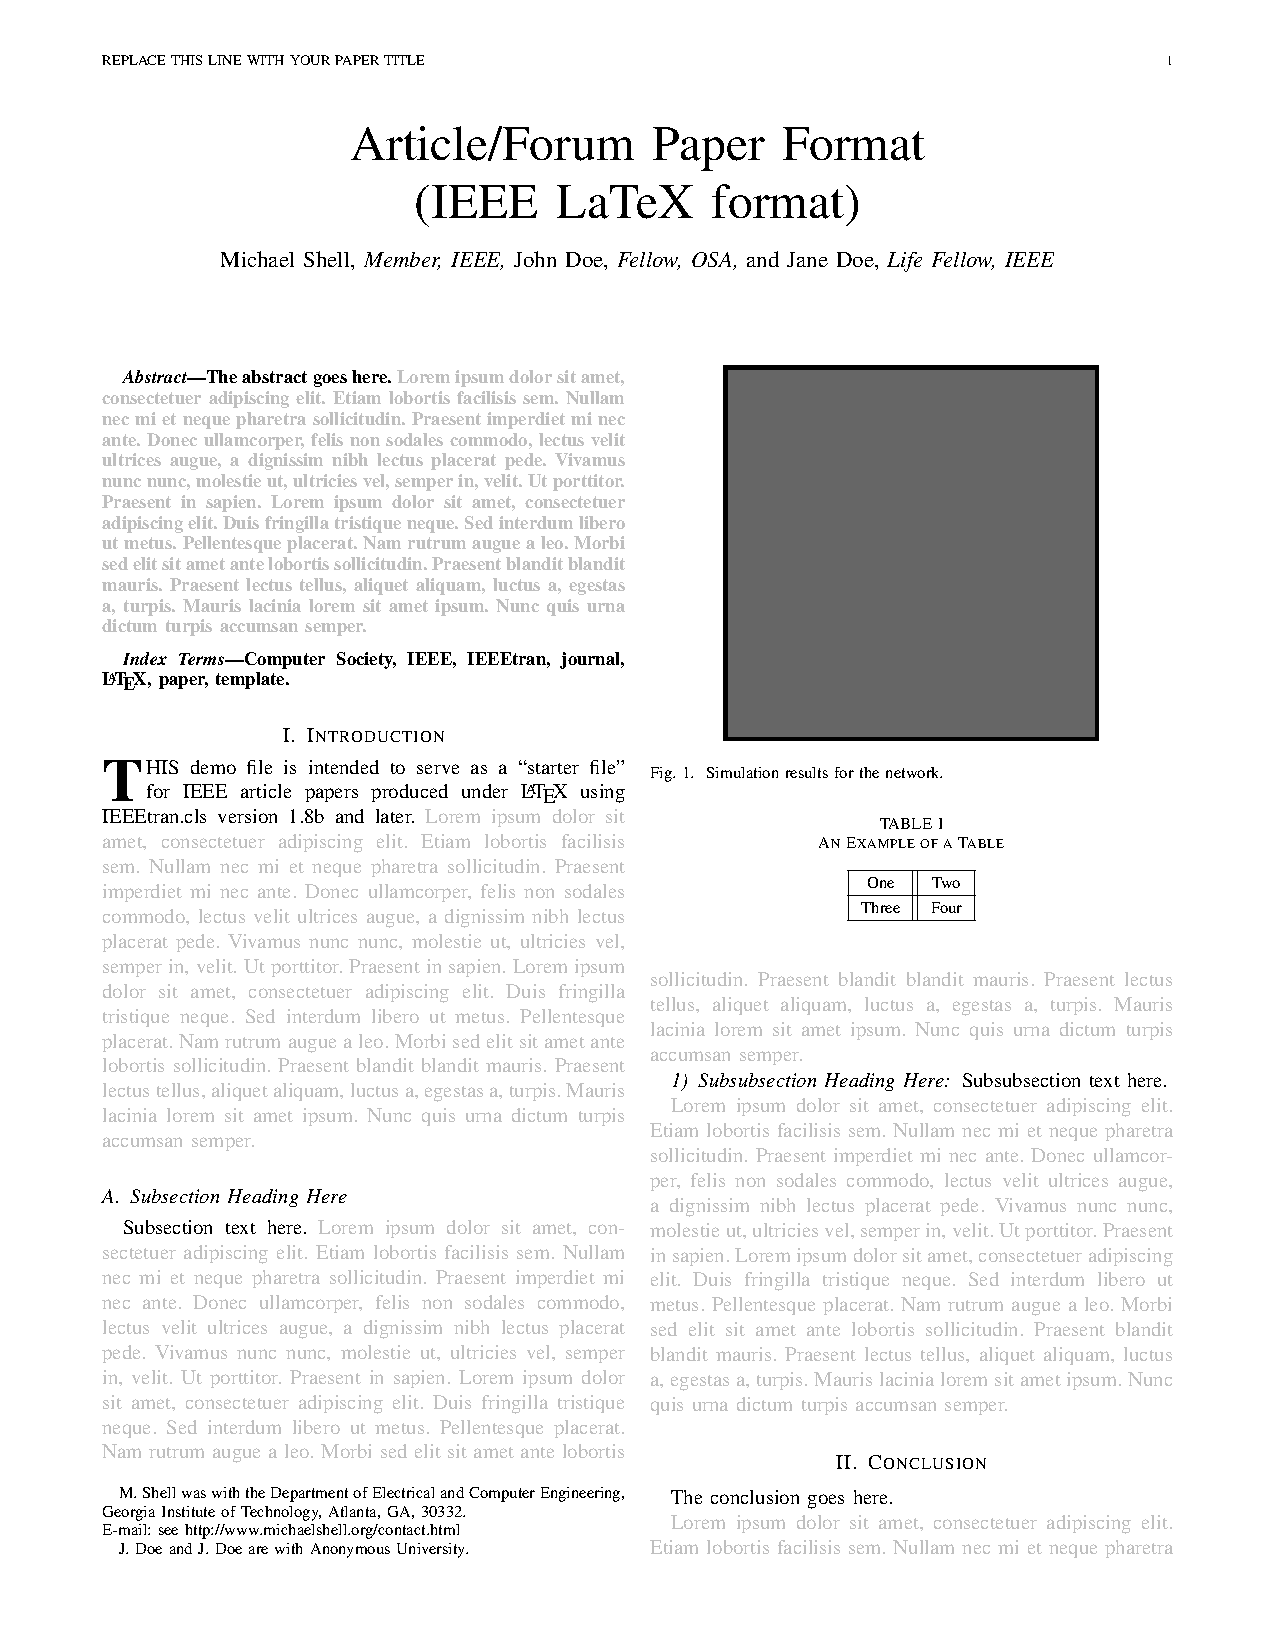
\includepdf[pages=-,%
	scale=1.0,%
	frame,%
	]
	{article_forum_paper.pdf}
	}
	\cleardoublepage

\end{document}